\documentclass[12pt,a4paper]{article}
\usepackage{inverba}

\newcommand{\userName}{Cullyn Newman} 
\newcommand{\class}{CH 334} 
\newcommand{\institution}{Portland State University} 
\newcommand{\theTitle}{\color{B-Cold} Organic Chemisty}

\begin{document}
%%%%%%%%%%%%%%%%%%%%%%%%%%%%%%%%%%%%%%%%%%%%%%%%%%%%%%%%%%%%%%%%%%%%%
\tableofcontents
\cleardoublepage
\fancyhead{}
\fancyhead[R]{\hyperlink{home}{\nouppercase\leftmark}}
%%%%%%%%%%%%%%%%%%%%%%%%%%%%%%%%%%%%%%%%%%%%%%%%%%%%%%%%%%%%%%%%%%%%%

\clearpage
%%%%%%%%%%%%%%%%%%%%%%%%%%%%% Chapter 1 %%%%%%%%%%%%%%%%%%%%%%%%%%%%%
%\begingroup
\clearpage
\section{General Chemistry Review}\phantomsection
\subsection{Electrons, Bonds, and Lewis Structures}
\begin{itemize}
    \item \textbf{Covalent bond}: two atoms sharing a pair of electrons.
    \item \textbf{Octet rule}: \textit{main group elements} that tend to bond in a way that each atom has {\color{o-Sun}eight} electrons in it's valence shell.
        \begin{itemize}
            \item Atoms that do not have eight will share electrons with other elements in order to maintain a stable state.
        \end{itemize}
    \item \textbf{Main group elements}: sometimes called representative elements, are groups 1, 2 and 13--18 in periodic table.
        \begin{itemize}
            \item Some elements in group 3 and 12 share properties between transition metals and the main group.
        \end{itemize}
    \item The lowest energy (most stable) state of two atoms is determined both by bond length and bond strength.
    \item Valence electrons are determined by the group, 1A--8A, of the periodic table.
    \item \textbf{Lone pair}: unshared, or nonbonding, electrons.
    \item \textbf{Lewis structures}: 2D model that represnets covalent bonds as straight lines and lonpairs as dots.
    \item Examples: \ch{COF2}, \ch{H2O}, \ch{NO3-}, \ch{N2O}:
        \begin{align*}
            \chemfig{C(=[2,.8]O)(-[5]F)(-[7]F)}
            \hspace{1cm}
            \chemfig{[:40]H-\lewis{13,O}-[::-80]H} 
            \hspace{1cm}
            \left[\chemfig{N(=[2,.8]O)(-[5]O)(-[7]O)}\right]^{-1} 
            \hspace{1cm}
            \chemfig{N(~[4]N)(-[0]O)}
        \end{align*}
    \item \textbf{Resonance structures}: a set of two or more Lewis structures that collectively describe the electronic bonding of a single polyatomic species, including fractional bonds.
    \subsubsection{Identifying Formal Charges}
    \begin{itemize}
    \item \textbf{Formal charge}: any atom that does not exhibit the appropriate number of valance electrons.
    \item Determining formal charge:
        \begin{itemize}
            \item Formula: {\color{o-Sun}\(FC = V - N - \dfrac{B}{2}\)}
            \item V = valance electrons of element
            \item N = lone pair electrons
            \item B = bonded electrons
        \end{itemize}
    \item {\color{pos}Less} than expected number of valence electrons results in a {\color{pos} positive} charge.
    \item {\color{neg}More} than expected number of valence electrons results in a {\color{neg}negative} charge.
    \item The lower the {\color{o-Sun}magnitude} of formal charge, the {\color{o-Sun}greater the stability} of the whole molecule.
    \item Atoms that are {\color{neg}more electronegative} hold {\color{neg}negative} formal charges better, which results in {\color{o-Sun}greater stability} vs when the negative charge is spread on less electronegative elements in a polyatomic species.
        \begin{itemize}
            \item The dominant resonance structure will be that of the greatest stability. 
        \end{itemize}
    \end{itemize}
\end{itemize}

\subsection{Induction and Polar Covalent Bonds}
\begin{itemize}
    \item Bonds can classified into three categories: covalent, polar covalent, and ionic.
    \item The categories emerge from the electronegativity values of the atoms sharing a bond.
    \item \textbf{Electronegativity}: a measure of the ability of an atom to attract electrons.
        \begin{itemize}
            \item Electronegativity generally {\color{o-Sun}increases left to right}, and from the {\color{o-Sun}bottom to top} of the periodic table.
            \item \textbf{F, O, N, Cl} (Br, I). Most electronegative elements, from left to right, that are often encountered.
        \end{itemize}
    \item \textbf{Covalent bond}: when the difference in electronegativity is {\color{o-Sun}less than 0.5}.
    \item \textbf{Polar covalent bond}: when the difference in electronegativity is {\color{o-Sun}between 0.5 and 1.9}, then the electrons are not equally shared and become polar.
    \item \textbf{Induction}: the withdrawl of electrons towards to more electronegative atom. {\color{pos}\ch{$\delta$^+}} represnets partial positive charged gained when electrons are pulled away, while {\color{neg}\ch{$\delta$^-}} represnets the partial negative charge pulled closer.
    \item \textbf{Ionic bond}: when the difference in electronegativity is {\color{o-Sun}greater than 1.9}.
        \begin{itemize}
            \item Electrons are not shared in this case, and attraction is insetsad just the result of oppositely charged ions.
        \end{itemize}
    \subsubsection{Dipole Moments and Molecular Polarity}
    \begin{itemize}
        \item \textbf{Dipole moment} ($\bm{\mu}$): defined as the amount of partial charge, $\delta$, on on either end of the dipole multiplied by the distance separtion, d:
             \begin{itemize}
                \item {\color{o-Sun}\(\mu=\delta d\)}
                \item $\mu$ generally has an order of magnitude of {\color{o-Sun}\SI{e-18}{esu.cm}} due to general partial charge (esu) and distance (cm) values.
                \item 1 {\color{o-Sun}debye (D)} = \SI{e-18}{esu.cm} 
             \end{itemize}
          \item \textbf{Molecular dipole moment}: the vector sum of the individual dipole moments.
              \begin{itemize}
                 \item Lone pairs have significant effect on the molecular dipole moment.
                 \item Also called the net dipole moment.
            \end{itemize}
    \end{itemize}
\end{itemize}

\subsection{Atomic Orbitals}
\begin{itemize}
    \item \textbf{Atomic orbital (AO)}: standing quantum wave (excitation in electron field) around an atom.
    \begin{itemize}
            \item More energy leads to higher orbtails levels.
                \begin{itemize}
                    \item Gives principle quantum number, \(n\), as is associated with distance from nucleus.
                \end{itemize}
            \item Orbital levels: s(1 pair), p(3 pairs), d(5 pairs), f(7 pairs). 
                \begin{itemize}
                    \item Angular momentum quantum number that describes three-dimensional region of space that the electron density occupies.
                \end{itemize}
            \item Magnetic quantum number descrices orientation in space of electron density.
                \begin{itemize}
                    \item \(m_l=0\); s orbital
                    \item \(m_l=-1, 0, 1\); p\(_{x}\), p\(_{y}\), p\(_{z}\) orbitals.
                \end{itemize}
            \item Locations where $\psi$ (quantum wave function) is zero are called \textbf{nodes}.
                \begin{itemize}
                    \item The {\color{o-Sun}more nodes} that an orbital has, the {\color{o-Sun}greater} it's energy.
                \end{itemize}
            \item \textit{Spin}: allows an orbital to contain only two electrons, \(\pm \frac{1}{2}\)
        \end{itemize}
    \item \textbf{Degenerate orbitals}: orbitals with the same energy level.
    \item Order in which orbitals are filled is determined by three principles:
        \begin{itemize}
            \item \textbf{Aufbau principle}: lowest energy orbital is filled first.
            \item \textbf{Pauli exclusion principle}: each orbital can accommodate a maximum of two electrons that have opposite spin.
            \item \textbf{Hund's rule}: electrons are placed in each degenerate orbital before being paired up.
        \end{itemize}
    \item Describing the nature of atomic orbital is done with two commoly used theories: \textit{Valence Bond Theory} and \textit{Molecular Orbital Theory}.
    \item The commonly used theories give a deeper understanding of covalent bonds, which is essentially just the {\color{o-Sun}overlap of atomic orbitals}.
    \item \textbf{Constructive/destructive interference}: the result of two waves that approach each other, or overlap.
        \begin{itemize}
            \item Constructive interference produces a wave with the vector sum of both waves.
            \item Destructive interference cancel each other out and produes a node.
        \end{itemize}

    \subsubsection{Valence Bond Theory}
    \begin{itemize}
    \item \textbf{Valence bond theory}: the sharing of electron density between two atoms is a result of the constructive interference of their atomic orbitals.
    \item \textit{Bond axis}: the line that can be drawn between two hydrogen atoms.
    \item \textbf{Sigma bond (\(\bm{\sigma}\))}: a particular type of covalent bond that has circular symmetry with respect to the bond axis.
        \begin{itemize}
            \item All single bonds are $\sigma$ bonds.
            \item The strongest type of covalent bond.
        \end{itemize}
    \item \textbf{Pi bond ($\bm{\pi}$)}: covalent bonds where two lobes of an orbital overlap with two lobes of another atom. 
        \begin{itemize}
            \item Each atomic orbital has zero electron density at a shared nodal plane, passing through the two bonded nuclei.
            \item $\pi$ bonds form double ($\sigma + \pi$) and triple bonds ($\pi + \sigma + \pi$).
            \item Individual $\pi$ bonds are weaker than $\sigma$ bonds.
        \end{itemize}
    \end{itemize}

    \subsubsection{Molecular Orbital Theory}
    \begin{itemize}
    \item \textbf{Molecular orbital theory (MO)}: uses linear combinations of atomic orbitals to model and explore the consequences of orbital overlap.
        \begin{itemize}
            \item The newly described orbitals are called {\color{o-Sun}molecular orbitals} accroding to MO theory.
        \end{itemize}
    \item Atomic orbitals refer to an individual atom, while molecular orbitals is associated with an entire molecular.
    \item In other words, MO theory states that atomic orbitals cease to exist when they overlap. Instead they are replaced with multiple molecular orbitals which span the entire molecule.
    \item Molecular orbitals are more stable (lower energy) since electrons are attracted by both nuclei.
    \item When there are {\color{o-Sun}nodes} between the nuclei, then the resulting $\sigma^*$ orbitals become {\color{o-Sun}antibonding}, as they {\color{o-Sun}destabilize} (increase the energy) of a molecular orbital.
    \item Best used to produce a quantitative picture of bonding.
        \begin{itemize}
            \item Describes strength, order, and polarity of bonds.
            \item Allows for the presence of paired or unpaired electrons.
            \item Has spectroscopic preperties.
        \end{itemize}
    \end{itemize}
    \subsubsection{Hybridized Atomic Orbitals}
\begin{itemize}
    \item \textbf{sp\(\bm{^3}\)-hybridized orbitals}: produced by averaging one \textit{s} orbital and {\color{o-Sun}three} \textit{p} orbitals.
        \begin{itemize}
            \item Hybridized orbitals explains to geomtry of methane, which results form the {\color{o-Sun}now four degenerate} orbitals pushing apart to achieve tetrahedral geometry.
            \item Hybridized orbitals become {\color{o-Sun}unsymmetrical}, producing a larger front lobe that is more efficient than standard \textit{p} orbitals in the ability to form bonds.
            \item All bonds in are {\color{o-Sun}$\sigma$ bonds}, and thus can be individually represented by the overlap of atomic orbitals.
        \end{itemize}
    \item \textbf{sp\(\bm{^2}\)-hybridized orbitals}: produced by averaging the \textit{s} orbital with only {\color{o-Sun}two} of \textit{p} orbitals.
        \begin{itemize}
            \item The remaining \textit{p} orbital is unaffected, and free multiple p orbitals results in a $\pi$ bond.
            \item This is done to expain geometry of compounds bearing a double bond.
            \item A double bond if formed from one $\sigma$ bond and one $\pi$ bond.
            \item Associated with \textit{trigonal planar geometry}.
        \end{itemize}
    \item \textbf{sp-hybridized orbitals}: produced by averaging of one \textit{s} orbital and {\color{o-Sun}one} \textit{p} orbital.
        \begin{itemize}
            \item Leaves two \textit{p} orbitals and resulting in two $\pi$ bonds.
            \item A triple bond is formed with the addition of one $\sigma$ bond due to the overlap of the sp orbitals.
            \item Geometry of a triple bond has \textit{linear geometry}.
        \end{itemize}
    \item Finding the hybridization of any atom can be done simply: 
        \begin{itemize}
            \item[1.] Look at the central item.
            \item[2.] Determine groups (number of bonds, $\pi$ bonds count as 1, and lone pairs attached) of atom.
                    \begin{itemize}
                        \item groups aka regions of electron density.
                    \end{itemize}
            \item[3.] For groups 1-4: sp\(^{x}\); x = groups - 1  
            \item[4.] For groups 5-6: sp\(^{3}\)d\(^{x}\); x = groups - 4 
        \end{itemize}
    \item Bond Strength and Bond Length:
        \begin{itemize}
            \item Bond length {\color{neg}decreases} with more bonds.
            \item Bond strength {\color{pos}increases} with more bonds.
            \item The more {\color{o-Sun}\textit{s} character}, the {\color{pos}shorter} and {\color{pos}stronger} the bond, and the {\color{pos}larger} the bond angle.
                \begin{itemize}
                    \item \textit{s-character}: contribution of the $\sigma$ bond in a hybridization.
                    \item e.g. sp = 50\%, sp\(^{2}\) = 33\%, sp\(^{3}\) = 25\%
                    \item sp-sp bond is the strongest, sp\(^{3}\)-sp\(^{3}\) is the weakest.
                \end{itemize}
        \end{itemize}
\end{itemize}
\end{itemize}

\subsection{Molecular Geometry}
\begin{itemize}
    \item \textbf{Valence shell electron pair repulsion (VSEPR) theory}: enables the {\color{o-Sun}prediction of molecular geometry} due to the pressumption that all electron pairs repel each other; resulting in a three-dimensional space that {\color{o-Sun}maximizes distance} from each other.
    \item \textbf{Steric number}: the total number of electron pairs in a molecule. Can be bonds or lone pairs.
    \item \textbf{Tetrahedral geometry}: result of four $\sigma$ bonds and zero lone pairs. 
        \begin{itemize}
            \item produces a tetrahendron with bond angles of \ang{109.5}.
        \end{itemize}
    \item \textbf{Trigonal pyramidal geometry}: three $\sigma$ bonds and one lone pair.
        \begin{itemize}
            \item The lone pair occupy more space than bonded electron pairs, so the remaining angles are slightly less than a tetrahedral, at \ang{107}.
            \item The lone pair sits atop the base forming a pyramid like structure.
        \end{itemize}
    \item \textbf{Bent geometry}: two $\sigma$ bonds and two lone pairs.
        \begin{itemize}
            \item VSEPR predicts the lone pairs to be in two corners of the tetrahedral, producing bond angles of \ang{105}.
            \item VSEPR predicts geometry \ch{H2O} correctly, but for wrong reasons.
                \begin{itemize}
                    \item The lone pairs in \ch{H2O} have different energy levels, suggesting one pair occupies a \textit{p} orbital with the other in a lower-energy hybridized orbital.
                \end{itemize}
        \end{itemize}
    \item VSEPR theory is best used for a first approximation and is mostly accurate for most small molecules.
    \item \textbf{Trigonal planar geometry}: three electron pairs forming three bond angles of \ang{120} and lie on the same plan. 
    \item \textbf{Linear geometry}: two electron pairs that oppose each other at \ang{180}, forming a linear structure.
    \item General method of determining structure:
    \begin{itemize}
        \item[1.] Count steric number---the total number of electron pairs in a molecule. Can be bonds or lone pairs.
        \item[2.] Determine predicted geomterical structure predicted (EDG) by VSEPR using steric number.
            \begin{itemize}
                \item Octahedral:6, Bipyramid:5, Tetrahedral:4, Trigonal:3, Linear:2
            \end{itemize}
        \item[3.] Determine impact (the MG) of lone pairs; more lone pairs results in less space between bonded pairs. Shape depends on EDG.
    \end{itemize} 
\end{itemize}


\subsection{Intermolecular Forces and Physical Properties}
\begin{itemize}
    \item \textbf{Intermolecular forces}: the attractive forces between individual molecules that determed the physical properties of a compound.
    \item \textit{Electrostatic}: forces that occur as a result of the attraction between opposite charges. 
    \item Electrostatic interactions for neutral molecules (no formal charge) are often classified as into the following categories:
        \begin{itemize} 
            \item \textbf{Dipole-dipole interaction}: Compounds with  {\color{o-Sun}net dipole} moments. 
                \begin{itemize}
                    \item In {\color{o-Sun}solid} space these intereactions either {\color{o-Sun}repel or attract} each other.
                    \item In {\color{o-Sun}liquid} space these interactions tend to {\color{o-Sun}attract more often}, raising melting/boiling point.
                    \item \textbf{Ion-dipole}: electrostatic interaction between an ion and a molecule with a dipole.
                \end{itemize}
            \item \textbf{Hydrogen bonding}: molecules with a hydrogen attached to an F, O, or N.
                \begin{itemize}
                    \item Not actually a bond, just an interaction.
                    \item When hydrogen bonds to a electronegative atom, then the hydrogen will have a {\color{pos}$\delta^+$}.
                    \item Hydrogen bonding is strong due to size of hydrogen atom, resulting in very close partial charge interactions.
                    \item The {\color{o-Sun}more} hydrogen bonds, the {\color{o-Sun}higher} the boiling point tends to be.
                    \item Stronger than dipole-dipole interactions.
                \end{itemize}
            \item \textbf{Fleeting dipole-dipole interactions}:
                \begin{itemize}
                    \item Electrons are considered to be in constant motion, which restult in the center of negative charge to vary.
                    \item \textbf{London Dispersion Forces (LDFs)}: On average, the dipole moment is zero, though it can experience transient dipole moments, initiating fleeting attraction/repulsion.
                        \begin{itemize}
                            \item All atoms and molecules have LDFs.
                            \item Weakest, but the dominant force in non-polar molecules.
                            \item Dispersion forces directly related to molar mass.
                        \end{itemize}
                    \item Heavier hydrocarbons generally experience a stronger force due to increased surface area, and thus greater chance for non-zero dipole moments, which results in higher boling points.
                    \item Branched hydrocarbons generally have decreased surface area, decreasing boiling point relative to others of similar weight.
                \end{itemize}
        \end{itemize}
    \item When comparing boling points of compounds, look for following factors:
        \begin{itemize}
            \item Any dipole-dipole interactions? (increases boiling point)
            \item Formation of hydrogen bonds? (increase boling point)
            \item Number of electrons. (more electrons, higher boiling point)
            \item Number of carbon atoms. (more surface area, higher boiling point)
            \item Degree of branching of compound. (more branching, more surface area)
        \end{itemize}
\end{itemize}
%\endgroup
%%%%%%%%%%%%%%%%%%%%%%%%%%%%% Chapter 1 %%%%%%%%%%%%%%%%%%%%%%%%%%%%%

%%%%%%%%%%%%%%%%%%%%%%%%%%%%% Chapter 2 %%%%%%%%%%%%%%%%%%%%%%%%%%%%%
%\begingroup
\clearpage
\section{Molecular Representations}\phantomsection
\subsection{Types of Molecular Representations}
\begin{itemize}
    \item \textbf{Partially condensed structures}: the \ch{C-H} bonds are not always drawn, saving space.
        \begin{itemize}
            \item \small\chemfig{C(-[4]CH_3)(-[2]OH)(-[0]CH_3)(-[6]H)}
        \end{itemize}
    \item \textbf{Condensed structures}: single bonds are not drawn and groups of atoms are clustered when possbile.
        \begin{itemize}
            \item \ch{CH3CH3CHOH -> (CH3)2CHOH}
        \end{itemize}
    \item \textbf{Molecular formula}: simply shows number of each type of atom with no structural information.
        \begin{itemize}
            \item \ch{C3H8O}
        \end{itemize}
    \item Example of converting a condensed structure into a partially condensed structure:
        \begin{itemize}
            \item ({\color{o-Sun}CH\(_{3}\)})\(_{3}\){\color{Liblue}CC}H\(_{2}\){\color{Liblue}C}H({\color{o-Sun}CH\(_{3}\)}){\color{Liblue}C}H({\color{o-Sun}CH\(_{3}\)}){\color{Liblue}C}H({\color{o-Sun}CH\(_{3}\)})\(_{2}\)
            \item \chemfig{{\color{Liblue}C}(-[4]{\color{o-Sun}CH_3})(-[6]{\color{o-Sun}CH_3})(-[2]{\color{o-Sun}CH_3})
            (-[0]{\color{Liblue}C}(-[6]H)(-[2]H)
            (-[0]{\color{Liblue}C}(-[6]{\color{o-Sun}CH_3})(-[2]H)
            (-[0]{\color{Liblue}C}(-[6]{\color{o-Sun}CH_3})(-[2]H)
            (-[0]{\color{Liblue}C}(-[6]{\color{o-Sun}CH_3})(-[2]H)(-[0]{\color{o-Sun}CH_3})
            ))))}
            \item This shows just one isomer, more partially condensed structures are possible.
        \end{itemize}

    \subsubsection{Bond-Line Structures}
    \begin{itemize}
        \item \textbf{Bond-line structures}; aka skeletal structures; simplify drawing process of chemical structures and are easier to read.
        \item Each corner or endpoint represents a carbon atom.
            \begin{itemize}
                     \item {\tiny\chemfig{-[:30]-[:-30]-[:30]-[:-30]-[:30]}
                     \hspace{15pt}
                     \chemfig{-[:30](-[:90])-[:-30]-[:30]-[:-30]}
                     \hspace{15pt}
                     \chemfig{-[:30](-[:90])-[:-30](-[:-90])-[:30]}}
                     \item All examples have 6 carbon atoms
            \end{itemize}
        \item Double bonds are shown with two lines, triple with three.
            \begin{itemize}
                \item {\tiny\chemfig{-[:30]=_[:-30]-[:30]}
                \hspace{15pt}
                \chemfig{-[:30]~[:30]-[:30]}}
                \item Triple bonds are drawn linearly due to sp-hybridization
            \end{itemize}
        \item Hydrogens are not shown; it is assumed that each carbon posses enough to satisfy octet rule.
    \end{itemize}
    \subsubsection{Notes on Drawing Bond-Line Structrues}
    \begin{itemize}
        \item Carbon atoms in a straight chain should be drawn in zigzag format in order to accurately show each carbon.
        \item Double bonds should be drawn as far apart as possible:
            \begin{itemize}
                \item {\tiny\chemfig{-[:30](=[:90]O)-[:-30]}} = good
                \hspace{20pt} {\tiny\chemfig{-[:30](=[:-90]O)-[:-30]}} = bad
            \end{itemize}
        \item Direction of a single bond is irrelevant:
            \begin{itemize}
                \item {\tiny\chemfig{-[:-30]-[:30](-[:90])-[:-30]-[:30]}}
                \hspace{12pt} is the same as \hspace{12pt} {\tiny\chemfig{-[:-90]-[:30](-[:90])-[:-30]-[:90]}}
                \item 
            \end{itemize}
        \item All {\color{o-Sun}heteroatoms} (atoms other than carbon and hydrogen) must be drawn.
            \begin{itemize}
                \item Hydrogens next to heteroatoms must be shown.
            \end{itemize}
        \item Carbons cannot have more than four bonds.
    \end{itemize}
\end{itemize}

\subsection{Hydrogen Deficiency Index: Degrees of Unsaturation}
{\color{G-Moon}\textit{Excerpt from Chapter 14: Infrared Spectroscopy and Mass Spectrometry}}
\begin{itemize}
    \item \textbf{Saturated compounds}: the maximum number of hydrogen atoms possbile, relative to number of carbon present.
        \begin{itemize}
            \item Determining saturation using molecular formula: {\color{o-Sun}C\(_{n}\)H\(_{2n+2}\)}~~\(n=\) carbon atoms
        \end{itemize}
            \begin{itemize}
                \item \textbf{Halogens}: takes the place of a hydrogen atom; {\color{o-Sun}add one H} for each halogen.
                \item \textbf{Oxygen}: no affect on saturation; {\color{o-Sun}ignore}.
                \item \textbf{Nitrogen}: needs an extra hydrogen; {\color{o-Sun}subtract one H} for each nitrogen. 
            \end{itemize}
    \item \textbf{Unsaturated compounds}: a compound that contains at least one $\pi$ bond, resulting fewer than the maximum number of hydrogen atoms.
        \begin{itemize}
            \item Compounds with rings also result in an unsaturated compound.
            \item \textbf{Degree of unsaturation}: a number that represnets {\color{o-Sun}half} the {\color{o-Sun}"missing"} number of hydrogen atoms when compared to a saturated compound.
        \end{itemize}
    \item \textbf{Hydrogen deficiency index (HDI)}: the measure of degrees of unsaturation. 
        \begin{itemize}
            \item e.g. two degrees of unsaturation results in a HDI of 2.
            \item Degrees of freedom help represent possbile structures, indicating possible double bounds, triple bounds, rings, or various combinations of each.
            \item Only helpful when molecular formula is known for certainty.
            \item Formula: {\color{o-Sun}HDI = \(\frac{1}{2}(2C + 2 + N - H - X)\)}
            \begin{itemize}
                \item \(X\): halogen atoms.
        \end{itemize}
    \end{itemize}
\end{itemize}

\subsection{Identifying Functional Groups}
\begin{itemize}
    \item \textbf{Functional group (R)}: specific substituents or moieties within molecules that may be responsible for the characteristic chemical reactions.
        \begin{itemize}
            \item \textbf{Substituents}: an atom or group of atoms which replaces one or more hydrogen atoms on the parent hydrocarbon chain.
            \item \textbf{Moiety}: a part of a molecule which is typically found within other molecules and often given a specific name.
        \end{itemize}
    \subsubsection{Characterizing Carbon Centers and Functional Groups}
    \begin{itemize}
        \item \textbf{Characterizing Carbon Centers}
            \begin{itemize}
                \item Primary \ang{1}: a carbon with only one carbon-carbon bond.
                    \begin{itemize}
                        \item \ch{H3C-CH3}\hspace{12pt}\chemfig{-[:30]\ang{1}}
                    \end{itemize}
                \item Secondary \ang{2}: a carbon with two carbon-carbon bonds.
                    \begin{itemize}
                        \item \ch{H3C-CH2-CH3}\hspace{12pt}\chemfig{-[:30]\ang{2}-[:-30]}
                    \end{itemize}
                \item Tertiary  \ang{3}: a carbon with 3 carbon-carbon bonds.
                    \begin{itemize}
                        \item \ch{(CH)3-CH}\hspace{12pt}\chemfig{-[:30]\ang{3}(-[:90])-[:-30]}
                    \end{itemize}
                \item Quaternary \ang{4}: a carbon with four carbon-carbon bonds.
                    \begin{itemize}
                        \item \ch{(CH)4-C}\hspace{12pt}\chemfig{-[:30]\ang{4}(-[:135])(-[:45])-[:-30]}
                    \end{itemize}
            \end{itemize}
        \item \textbf{Characterizing Functional Groups}
            \begin{itemize}
                \item Certain functional groups can be characters as \ang{1}, \ang{2}, or \ang{3}, based on how many carbon bonds are attached to the carbon with the functional group.
            \end{itemize}
    \end{itemize}
\end{itemize}

\subsection{Identifying Lone Pairs}
\begin{itemize}
    \item Formal charges must always be drawn on bond line structures, otherwise the resulting bond line strcutres would be inferred incorrectly.
    \item Lone pairs do not have to be drawn and usually are omitted.
    \item The formal charge allows you to determine lone pairs.
        \begin{itemize}
            \item Formula: \(FC = V - N - \dfrac{B}{2}\)
            \item V = valance electrons of element
            \item N = lone pair electrons
            \item B = bonded electrons
            \item Solve for lone pairs: {\color{o-Sun}\(N = V - FC - \dfrac{B}{2}\)}
        \end{itemize}
    \item Frequent usage will allow for intuition for lone pairs.
    \newpage
    \subsubsection{Common Patterns Between Formal Charge and Lone Pairs}
    \begin{itemize}
        \item \textbf{Associated Patterns for Oxygen}
            \begin{itemize}
                \item A {\color{neg}negative ($\circleddash$)} charge corresponds with {\color{o-Sun}1 bond} and {\color{o-Sun}3 lone pairs}.
                \item The {\color{G-Moon}absence} of charge corresponds with {\color{o-Sun}2 bonds} and {\color{o-Sun}2 lone pairs}.
                \item A {\color{pos}positive ($\oplus$)} charge corresponds with {\color{o-Sun}3 bonds} and {\color{o-Sun}1 lone pair}.
            \end{itemize}
        \item \textbf{Associated Patterns for Nitrogen}
            \begin{itemize}
                \item A {\color{neg}negative} charge corresponds with {\color{o-Sun}2 bonds} and {\color{o-Sun}2 lone pairs}.
                \item The {\color{G-Moon}absence} of charge corresponds with {\color{o-Sun}3 bonds} and {\color{o-Sun}1 lone pair}.
                \item A {\color{pos}positive} charge corresponds with {\color{o-Sun}4 bonds} and {\color{o-Sun}0 lone pairs}.
            \end{itemize}
    \end{itemize}
\end{itemize}

\subsection{Resonance}
\begin{itemize}
    \item \textbf{Resonance}: description of bonding in molecules or ions by the combination of multiple contributing strcutres.
            \begin{itemize}
            \item \textbf{Resonance structures}: each contributing structure of the resonance hybrid.
                \begin{itemize}
                    \item Formal charges are important to include when drawing resonance structures as it clarifies where locations of lone pairs and movement of electrons.
                    \item Total charge must remain the same between structures.
                \end{itemize}
        \end{itemize}
    \item Resonance does not describe any real process, rather it's a method to overcome inadequacy of bond-line drawings.
    \item Different from isomerism, which differs in arrangements of atomic nuclei in space, rather than how the electrons are assigned to the depictions.
    \subsubsection{Resonance: Curved Arrows}
    \begin{itemize}
        \item \textbf{Curved arrows}: a tool used to help draw resonance strcutres by {\color{o-Sun}representing electrons as if} they were moving.
            \begin{itemize}
                \item Somwhat different from curved arrow notation in reactions, which actually represent the flow of electron density.
                \item Can help shows how to change the formal charge:
                    \begin{itemize}
                        \item Formal charges at the {\color{o-Sun}tail} become more {\color{pos}positive}, since it's losing an electron.
                        \item Formal charges at the {\color{o-Sun}head} more {\color{neg}negative}, since it's gaining an electron.
                    \end{itemize}
            \end{itemize}
        \item {\color{o-Sun}Avoid breaking a single bond}.
            \begin{itemize}
                \item Structures must have atoms connected in same order, though there are minor exceptions that \textit{will be discussed later}.
                \item This rule affects the placement of the {\color{o-Sun}tail} of the arrow, as it represents distribution of previous electrons.
            \end{itemize}
        \item {\color{o-Sun}Never exceed an octet for second-row elements}.
            \begin{itemize}
                \item Not a violation to have less than an octet. 
                \item This rule affects the placement of the {\color{o-Sun}head} of the arrow, as it represents sharing of new electrons.
            \end{itemize} 
        \item Can only be used on adjcent atoms, though the electrons 
        can be pushed multiple times.
        \item "Legal" moves: 
            \begin{itemize}
                \item $\pi$ bond $\rightarrow$ lone pair. 
                \item Lone pair $\rightarrow$ $\pi$ bond.
                \item $\pi$ bond $\rightarrow$ $\pi$ bond.
                \item Every resonance structure can be built through a combination of above three moves.
            \end{itemize}
    \end{itemize}
    \subsubsection{Common Patterns of Resonance Structures}
    \begin{itemize}
        \item \textbf{Vinylic}: the two carbon atoms bearing the double bond of a carbon-carbon double bond.
        \item \textbf{Allylic}: atoms connected directly to vinylic positions.
    \end{itemize}
    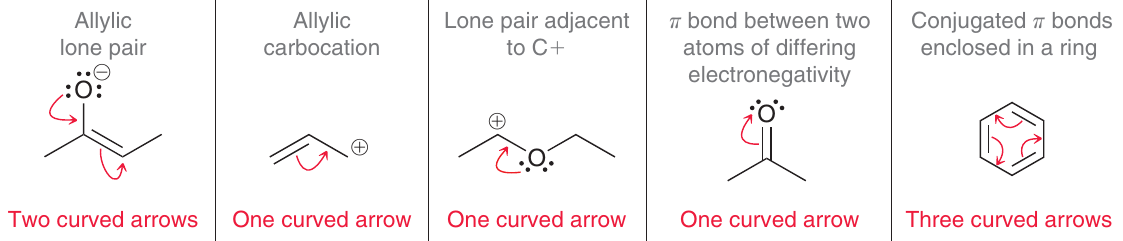
\includegraphics[width=\linewidth]{images/patterns.png}
    \subsubsection{Resonance Hybrid}
    \begin{itemize}
        \item \textbf{Resonance hybrid}: respresents the \textit{average} of the contributing structures, with bond lengths and partial charges taking on intermediate values.
        \item No matter how many resonance structures are drawn, they collectively represent one entity.
        \item Drawn partial bonds and charges to illustrate the delocalization of electrons.
    \end{itemize}
    \subsubsection{Delocalization}
    \begin{itemize}
        \item \textbf{Delocalization}: the spreading of electrons between multiple atoms or covalent bonds.
        \begin{itemize}
            \item \textbf{Resonance stabilization}: molecules and ions that are {\color{o-Sun}stabliized} by the delocalization of electrons.
            \item Plays a major role in the outcome of many reactions.
        \end{itemize}
 with         \item When a lone pair particpates in resonance, it will occupy a \textit{p} orbtail rather than hybridized; important for 3d shapes of proteins.
        \item \textbf{Localized lone pair}: when a lone pair is not allylic to a $\pi$ bond. 
            \begin{itemize}
                \item Whenever an atom posses both a $\pi$ bond and a lone pair, they will not both participate in resonance.
                \item Usually $\pi$ bonds participate first.
            \end{itemize}
    \end{itemize}
    \subsubsection{Contributor Significance}
    \begin{itemize}
        \item Some resonance structures may resemble the actual molecule more than another, in regards to energy and stability.
        \item Strcures with low potential energy are more stable compared to those of higher values and resemble the actual structure more.
        \item \textbf{Major contributors}: the most stable contributing structures.
        \item \textbf{Minor contributors}: less favorable contributing strcutres.
        \item Rules for contributing significance, descending:
            \begin{itemize}
                \item The greatest number of filled octets.
                \item The greatest number of covalent bonds.
                \item Minimize formally charged atoms.
                \item Separation of unlike and like charges, minimized and maximized respectively.
                \item Negative charges placed on the most electronegativity atoms, positive charges placed on the less electronegative atoms.
                \item Do not deviate substantially from idealized bond lengths and angles.
                \item Maintain aromatic substructures locally while avoiding anti-aromatic ones.
            \end{itemize}
    \end{itemize}
\end{itemize}
%\endgroup
%%%%%%%%%%%%%%%%%%%%%%%%%%%%% Chapter 2 %%%%%%%%%%%%%%%%%%%%%%%%%%%%%

%%%%%%%%%%%%%%%%%%%%%%%%%%%%% Chapter 3 %%%%%%%%%%%%%%%%%%%%%%%%%%%%%
%\begingroup
\clearpage
\section{Acids and Bases}\phantomsection
\subsection{Br{\o}nsted-Lowry Acids and Bases}
\begin{itemize}
    \item \textbf{Acid}: a {\color{o-Sun}proton donor}; i.e., a {\color{pos}\ch{H^+}} donor.
    \item \textbf{Base}: a {\color{o-Sun}proton acceptor}; i.e., a {\color{neg}\ch{OH^-}} (hydroxide ion), which wants a {\color{pos}\ch{H^+}} to form the more stable \ch{H2O}.
    \item General definition: {\color{pos}acid} + {\color{neg}base} \ch{<>} {\color{neg}conjugate base} + {\color{pos}conjugate acid}
        \begin{itemize}
            \item Symbolically: {\color{pos}HA} + {\color{neg}B} \ch{<>} {\color{neg}\ch{A^-}} + {\color{pos}\ch{HB^+}}
            \item The strength of the acid/base is {\color{o-Sun}inversley proportional} to the strength of the conjugate acid/base.
        \end{itemize}
    \item Most acid-base reactions are reversible.
        \begin{itemize}
            \item Strong acids tend to be less reversible.
        \end{itemize}
    \item Example using bond-line structures:
        \begin{itemize}
            \item 
            \chemfig{{\color{pos}H}-[:30]O-[:-30]H}
            \hspace{6pt}{\large+}\hspace{6pt}
            \chemfig{-[:30](-[:120])(-[:60])-[:-30]\chemabove{\textcolor{neg}O}{{\color{neg}\scriptstyle\circleddash}}} 
            \hspace{6pt}{\large\ch{<>}}\hspace{6pt}
            {\color{neg}$^\circleddash$O}H
            \hspace{6pt}{\large+}\hspace{6pt}
            \chemfig{-[:30](-[:120])(-[:60])-[:-30]O-[:30]{\color{pos}H}}
    \end{itemize}
    \subsubsection{Quantitative Perspective}
    \begin{itemize}
        \item \textbf{Equilibrium}: when there is no longer an observable change in concentrations of reactants and products.
            \begin{itemize}
                \item \(K_{eq}=\dfrac{[\ch{H3O+}]\,[\ch{A-}]}{[\ch{HA}]\,[\ch{H2O}]}\)
                \item Water concentration is fairly constant and can be removed, giving \(K_a\).
                    \begin{itemize}
                        \item \(K_a=K_{eq}\,[\ch{H2O}]=\dfrac{[\ch{H3O+}]\,[\ch{A-}]}{[\ch{HA}]}\)
                    \end{itemize}
                \item \(K_a\) tends to be large, so it's converted to \(pK_a\).
                    \begin{itemize}
                        \item \(pK_a=-\log{K_a}\)
                        \item Generally ranges from {\color{pos}-10 (strong acid)} to {\color{neg}50 (strong base)}.
                    \end{itemize}
                \item {\color{pos}\(pK_a\) (\ch{H+})} can be easily converted to {\color{neg}\(pK_b\) (\ch{OH-})}:
                    \begin{itemize}
                        \item \(pK_b=14-pK_a\)
                    \end{itemize}
            \end{itemize}
        \item Equilibrium {\color{o-Sun}favors formation} of the {\color{o-Sun} weaker} (higher \(pK_a\)) {\color{o-Sun}acid}.
            \begin{itemize}
                \item Reactions with vastly different \(pK_a\) values make the reverse proccess is negligible.
                \item Can ignore the reverse reaction in such cases and treat it as a reaction in one direction.
            \end{itemize}
    \end{itemize}
    \subsubsection{Qualitiative Perspective}
    \begin{itemize}
        \item Relative acid strength can be determined by comparing conjugate bases. 
            \begin{itemize}
                \item The {\color{o-Sun}more stable} (weaker) the conjugate base, the {\color{o-Sun}stronger} the acid.
                \item Does not predict \(pK_a\), just a means of comparing relative acid strenghts with out known \(pK_a\)
            \end{itemize}
        \item \textbf{Stabilization factors}: (1) {\color{o-Sun}atom bearing the charge}, (2) {\color{o-Sun}resonance}, (3) {\color{o-Sun}induction}, and (4) {\color{o-Sun}orbitals}.
            \begin{itemize}
                \item Generally follow decending order of significance; absence of difference in earlir factors allow for later factors to express more significance.
            \end{itemize}
        \item \textbf{Atom bearing the charge}: Compare atoms bearing negative charge in each conjugate base after deprotonation.
            \begin{itemize}
                \item First determine if atoms are in same row or column in the periodic table.
                \item {\color{o-Sun}Row} comparison: {\color{o-Sun}electronegativity} is the dominant effect; stability is greater when the negative charge is on the {\color{o-Sun}more electronegative} element.
                \item {\color{o-Sun}Column} comparsion: {\color{o-Sun}size} is the dominant effect; stability is greater when the negative charge is on the {\color{o-Sun}larger} element. 
            \end{itemize}
        \item \textbf{Resonance}: charge that is delocalized across multiple atoms will lead to more stable structures comapred to molecules with no resonance.
            \begin{itemize}
                \item Helps determining relative stability when both molecules bare the same elements that have a difference in charge.
                \item Again, more stability means it's the weaker conjugate base, meaning the proton removed from the atom creating the resonance hybrid will be more acidic.
            \end{itemize}
        \item \textbf{Induction}: induction of other atoms can act to withdraw the negative charge away from the new electronegatively charged atom due to deprotonation.
            \begin{itemize}
                \item Inductive effect diminishes the further the electronegative atom is away from the depronated atom.
            \end{itemize}
        \item \textbf{Orbitals}: negative charges on atoms with lower hybridization result in greater stability due to proximity to positive nucleus, i.e., \({\color{neg}sp} > sp^2 > {\color{pos}sp^3}\)
            \begin{itemize}
                \item sp = triple bond, sp\(^{2}\) = double bond, sp\(^{3}\) = three $\sigma$ bonds.
            \end{itemize}
    \end{itemize}
\end{itemize}

\subsection{Lewis Acids and Bases}
\begin{itemize}
    \item The lewis definition is more broad than the Br{\o}nsted-Lowry definition.
    \item Lewis describes acidity in terms of {\color{o-Sun}electrons}, rather than protons.
    \item \textbf{Lewis acid}: electron-pair {\color{o-Sun}acceptor}.
    \item \textbf{Lewis base}: electron-pair {\color{o-Sun}donor}.
    \item All B{\o}nsted-Lowry acids and bases are Lewis acid and bases, but the inverse is not always true.
    \item Most reactions are described in terms of lewis base and acids, since molecules without donatable protons are unable to be described by the Br{\o}nsted-Lowry definition.
\end{itemize}

\subsection{Nucleophiles and Electrophiles}\label{ssec:bar}
{\color{darklc}\textit{Excerpt from Chapter 6: Chemical Reactivity and Mechanisms $\mapsto$}}\label{Nucleophiles and Electrophiles}

{\color{darklc}{\color{G-Moon}\nameref{Mechanisms and Arrow Puhsing}} may also be useful}.
\begin{itemize}
    \item \textbf{Ionic reactions}, {\color{G-Moon}aka polar reactions}: reactions that involve the particpation of ions as reactants, intermediates, or products.
        \begin{itemize}
            \item Most cases ions act as intermediates.
            \item Radical reactions and pericyclic reactions are also major categories, but are typically not discussed in undergraduate courses.
            \item Ionic reactions occur when one reactant has a site of {\color{neg}high electron density} and the other reactant has a site of {\color{pos}low electron density}.
        \end{itemize}
    \item \textbf{Nucleophiles}: an electron rich atom that is capable of donating a pair of electrons.
        \begin{itemize}
            \item {\color{neg}Lewis bases are nucleophiles}, but not all nucleophiles are lewis bases.
            \item Any atom that possesses a localized lone pair can be nucleophilic.
            \item $\pi$ bonds can also function as nucleophiles due to their region of space having high electron density.
        \end{itemize}
    \item \textbf{Electrophiles}: an electron-deficient atom that is capable of accepting a pair of electrons.
        \begin{itemize}
            \item {\color{pos}Lewis acids are electrophiles}, but not all electrophiles are lewis acids.
        \end{itemize}
\end{itemize}

\subsection{Flow of Electron Density: Curved-Arrow Notation}
\begin{itemize}
    \item All reactions are accomplished via a flow of electron density.
    \item Electron density flow is illustrated with curved arrows.
        \begin{itemize}
            \item \textbf{Reaction mechanism}: how the reaction occurs in terms of the motion 
            \item All ionic meachanisms, regardless of complexity, are combinations of four characteristic patterns of electron flow \textit{(discussed later)}.
        \end{itemize}
    \subsubsection{Notes on Drawing Curved Arrows}
    \begin{itemize}
        \item \textbf{Tails} must be placed on either a bond or a lone pair.
            \begin{itemize}
                \item Shows the {\color{o-Sun}source}, i.e., the electron donor (base).
                \item Electrons can only be found in lone pairs or bonds, so {\color{o-Sun}never place the tail} of a curved arrow on a {\color{pos}positive charge}.
            \end{itemize}
        \item \textbf{Heads} must be placed so that it shows either the formation of a bond or the formation of a lone pair.
            \begin{itemize}
                \item Shows the {\color{o-Sun}destination}, i.e., the electron acceptor (acid).
                \item Avoid drawing an arrow that violates the octet rule, so never draw an arrow that gives more than four orbitals to a second-row element.
            \end{itemize}
    \end{itemize}
\end{itemize}

%\endgroup
%%%%%%%%%%%%%%%%%%%%%%%%%%%%% Chapter 3 %%%%%%%%%%%%%%%%%%%%%%%%%%%%%

%%%%%%%%%%%%%%%%%%%%%%%%%%%%% Chapter 4 %%%%%%%%%%%%%%%%%%%%%%%%%%%%%
%\begingroup
\clearpage
\section{Alkanes and Cycloalkanes}\phantomsection
\subsection{Nomenclature of Alkanes}
\begin{itemize}
    \item \textbf{Alkane}: acyclic (linear structure) saturated hydrocarbons (no $\pi$ bonds).
        \begin{itemize}
            \item General chemical formula: {\color{o-Sun}\ch{C_nH_{2n+2}}}
        \end{itemize}
    \item \textbf{Substituents}: branches connected to the parent chain.
    \subsubsection{Selecting the Parent Chain}
    \begin{itemize}
        \item \textbf{Parent chain}: the longest carbon chain in an alkane.
        \begin{table}[h]
            \centering
            \caption{Parent Names for Alkanes\strut}
            \label{tab:alkanes}
            \begin{tabular}{ccc}
                \toprule
                Number of Carbons & Parent & Name \\
                \midrule
                1 & meth & methane \\
                2 & eth & ethane \\
                3 & pro & propane \\
                4 & but & butane \\
                5 & pent & pentane\\
                6 & hex & hexane \\
                7 & hept & heptane \\
                8 & oct & octane \\
                9 & non & nonane \\
                10 & dec & decane \\
                11 & undec & undecane \\
                12 & dodec & dodecane \\
                13 & tridec & tridecane \\
                14 & tetradec & tetradecane \\
                15 & pentadec & pentadecane\\
                20 & eicos & eicosane \\
                30 & triacont & triacontane \\
                40 & tetracont & tetracontane \\
                50 & pentacont & hectane \\
                100 & hect & hectane \\
                \bottomrule
                \end{tabular}
        \end{table}   
    \item \textbf{Substituents}: branches connected to the parent chain, can be a single atom, groups of atoms, that replace one or more hydrogen atoms. 
        \begin{itemize}
            \item If there is competition between chains of {\color{o-Sun}equal length}, then {\color{o-Sun}choose the chain with greatest number of substituents}.
        \end{itemize}
    \item \textbf{Cycloalkanes (cyclo)}: presence of a ring in an alkane.
    \end{itemize}
    \subsubsection{Naming Substituents}
    \begin{itemize}
        \item \textbf{Alkyl groups}: Substituents that are named the same as the parents, but with the added letters {\color{o-Sun}ly}.
        \begin{table}[h]
            \centering
            \caption{Names of Alkyl Groups\strut}
            \label{tab:substituents}
            \begin{tabular}{ccc}
                \toprule
                Substituent Carbons&  Terminology\\
                \midrule
                1 & meth{\color{o-Sun}y}l\\
                2 & eth{\color{o-Sun}yl} \\
                3 & pro{\color{o-Sun}pyl} \\
                4 & but{\color{o-Sun}yl} \\
                5 & pent{\color{o-Sun}yl} \\
                6 & hex{\color{o-Sun}yl} \\
                7 & hept{\color{o-Sun}yl} \\
                8 & oct{\color{o-Sun}yl} \\
                9 & non{\color{o-Sun}yl} \\
                10 & dec{\color{o-Sun}yl} \\
                \bottomrule
                \end{tabular}
        \end{table}
        \item When a group is connected to the ring, then the ring is generally treated as the parent.
            \begin{itemize}
                \item If the ring has fewer atoms the the rest of the structure, then it becomes a substituent.
            \end{itemize}
    \end{itemize}
    \subsubsection{Naming Complex substituents}
    \begin{itemize}
        \item \textbf{Complex substituents}: branched alkyl substituents.
        \item Begin by numbering carbons going {\color{o-Sun}away} from the parent chain, then name it as if its a parent chain itself.
            \begin{itemize}
                \item Complex substituent are placed in parentheses, indicating it as a single substituent of the parent chain.
            \end{itemize}
        \item Some complex substituents have common names that are so well established and allowed by IUPAC.
            \begin{itemize}
                \item An alkyl group bearing {\color{o-Sun}three} carbon atoms; only one way to branch it.
                    \begin{itemize}
                        \item \textbf{Isopropyl group}: (1-methylethyl): {\tiny\chemfig{-[:0](-[::60])-[::-60]}}
                    \end{itemize}
                \item Alkyl groups bearing {\color{o-Sun}four} carbon atoms, which can be branched three different ways:
                    \begin{itemize}
                        \item \textbf{sec-butyl} (1-methylpropyl): {\tiny\chemfig{-[:0](-[::60]-[:0])-[::-60]}}
                        \item \textbf{isobutyl} (2-methylpropyl): {\tiny\chemfig{-[:0](-[::60](-[:120])-[:0])}}
                        \item \textbf{tert-butyl} (1,1-dimethylethyl): {\tiny\chemfig{-[:0](-[::60])(-[:0])(-[::-60])}} 
                    \end{itemize}
                \item Alkyl groups bearing {\color{o-Sun}five} carbons, which can be branched many more ways. Two common ways:
                    \begin{itemize}
                        \item \textbf{isopentyl (isoamyl)} (3-methylbutyl): 
                    {\tiny\chemfig{-[:0]-[::60]-[:0](-[:60])-[:-60]}}
                        \item \textbf{neopentyl} (2,2-dimethylpropyl):
                    {\tiny\chemfig{-[:0]-[::60](-[:-15])(-[:50])(-[:120])}}
                    \end{itemize}
            \end{itemize}
    \end{itemize}
    \subsubsection{Assembling the Systematic Name}
    \begin{itemize}
        \item \textbf{Locant}: the location of a carbon numbered parent chain.
        \item Rules for assinging locant:
            \begin{itemize}
                \item If one substituent is present, then assign the lowest number possbile.
                \item When multiple substituents are present, then the first substituent receives the lowest number. 
                    \begin{itemize}
                        \item If there is a tie, the second locant should be as low as possible.
                        \item If tie cannot be broken, then lowest number is assigned alphabetically.
                    \end{itemize}
                \item Prefixes are used when the same substituent appears more than once. 
                    \begin{itemize}
                        \item di:2, tri:3, tetra:4, penta:5, 6:hexa
                    \end{itemize}
                \item Hypens are used to separate numbers from letters, while commas are used to separate numbers from each other.
                \item Substituents are alphabeticalized after all locants are correctly assigned.
                    \begin{itemize}
                        \item Prefixes are ignored during alphabeticalization.
                    \end{itemize}
            \end{itemize}
        \item Summary of discrete steps:
            \begin{enumerate}
                \item \textbf{Identify parent chain}
                \item \textbf{Identify and name substituents}
                \item \textbf{Number the parent chain and assign a locant to each substituent}
                \item \textbf{Arrange the substituents alphabetically}
            \end{enumerate}
    \end{itemize}
\end{itemize}

\subsection{Constitutional Isomers of Alkanes}
\begin{itemize}
    \item For an alkane, the number of possible constitutional isomers increases with increaseing molecular size.
    \item Determining IUPAC name is the best way to tell if two alkanes are constitutional isomers, or just different representations of the same one.
    \begin{table}[h]
        \centering
        \caption{Constitutional Isomers for Various Alkanes\strut}
        \label{tab:constitutional}
        \begin{tabular}{ccc}
            \toprule
            Molecular Formula &  Constitutional Isomers\\
            \midrule
            \ch{C3H8} & 1\\
            \ch{C4H10} & 2\\
            \ch{C5H12} & 3\\
            \ch{C6H14} & 5\\
            \ch{C7H16} & 9\\
            \ch{C8H18} & 18\\
            \ch{C9H20} & 35\\
            \ch{C10H22} & 75\\
            \ch{C15H32} & 4,347\\
            \ch{C20H42} & 366,319\\
            \ch{C40H62} & 4,111,846,763\\
            \bottomrule
            \end{tabular}
    \end{table}
\end{itemize}

\subsection{Newman Projections}
\begin{itemize}
    \item \textbf{Conformations}: the variety of possible three-dimensional shapes of a molecule that are interchangeable by low energy pathways.
        \begin{itemize}
            \item Conformations vary in potential energy.
            \item Changes due to rotation about $\sigma$ bonds.
        \end{itemize}
    \item \textbf{Configurations}: refer to different orientations in space that require breaking of bonds (high energy pathway) to change.
        \begin{itemize}
            \item Cis and trans isomers in alkenes (\textit{discussed later})
        \end{itemize}
    \item \textbf{Newman projections}: a type of representation of compounds specially designed for showing the conformation of a molecule.
        \begin{itemize}
            \item Drawn from the angle of the observer, with the front carbon represented in front of the circle, and the back carbon behind the circle.
            \item ***Chemmacros package is broken due to font usage, need to figure out how to fix that before inserting drawings***
        \end{itemize}
    \subsubsection{Conformational Analysis of Ethane and Propane}
    \begin{itemize}
        \item \textbf{dihedral (torsional) angle}: the angle between substituents of front and back carbons as the $\sigma$ bonds rotates.
        \item There are an infinite number of possbile conformations, but there are conformations of maximum and minium energy.
            \begin{itemize}
                \item \textbf{Staggered conformation}: {\color{o-Sun}lowest energy} conformation, when two substituents are at maximum dihedral angle from each other.
                \item \textbf{Eclipsed conformation}: the {\color{o-Sun}highest energy} conformation, when two substituents are at the minimum dihedral angle from each other.
            \end{itemize}
        \item \textbf{Degenerate}: when all staggered conformations have the same amount of energy.
            \begin{itemize}
                \item All staggered and eclipsed conformations of ethanes are degenerate.
            \end{itemize}
        \item \textbf{Torsional strain}: the difference in energy between staggered and eclipsed conformations.
            \begin{itemize}
                \item Recent quantum methods suggest conformation possesses a favorable interaction between occupied, bonding molecular orbitals and unoccupied, antibonding molecular orbitals.
                \item An increase in potential energy occurs when the favorable overalp is broken.
                \item A sample of ethane gas at room temperature will have \(\approx\) 99\% of its molecules staggered.
            \end{itemize}
        \item Ethane has total cost of \SI{12}{kJ\per\mole} (\SI{4}{kJ\per\mole\per H}), while propane has total cost of \SI{14}{kJ\per\mole}.
            \begin{itemize}
                \item Reasonable estimates of energy cost of an H eclipsing a \ch{CH3} group must be \SI{6}{kJ\per\mole}.
            \end{itemize}
    \end{itemize}
    \subsubsection{Conformational Analysis of Butane}
    \begin{itemize}
        \item Butane has three eclipsed conformations that are {\color{o-Sun}not degenerate}.
            \begin{itemize}
                \item Dihedral angle of \ang{0} has the highest eclipsed energy, while both conformations at \(\pm\)\ang{120} are second highest in energy and degenerate.
                \item Likewise, a dihedral angle of \ang{180} has the lowest staggered energy, while both conformations at \(\pm\)\ang{60} are second lowest in energy and degenerate.
            \end{itemize}
        \item \textbf{Anti conformation}: the conformation with a dihedral angle of \(180\); the lowest staggered energy.
            \begin{itemize}
                \item Occurs when the methyl groups are farthest apart.
            \end{itemize}
        \item \textbf{Steric interaction}: nonbonding intereactions that influences energy levels conformations.
        \item \textbf{Gauche interaction}: unfavorable intereaction between substituents, causing an increases in energy due to electron cloud repulsion.
            \begin{itemize}
                \item Gauche intereaction is a type of steric intereactions present at \(\pm\ang{60}\) of the next eclipsed conformation.
            \end{itemize}
        \item Costs of butane: \SI{19}{kJ\per\mole}, \SI{16}{kJ\per\mole}, \SI{3.8}{kJ\per\mole}
            \begin{itemize}
                \item Energy cost of eclipsing \ch{CH3}/\ch{CH3}: \SI{11}{kJ\per\mole}
                \item Energy cost for gauche interaction of \ch{CH3}/\ch{CH3} \SI{3.8}{kJ\per\mole} for butane.
                \item Energy cost of eclipsing \ch{CH3}/H: \SI{6}{kJ\per\mole} 
                \item Energy cost of eclipsing H/H: \SI{4}{kJ\per\mole} 
            \end{itemize}
    \end{itemize}
\end{itemize}

\subsection{Cycloalkanes}
\begin{itemize}
    \item \textbf{Angle strain}: the increases in energy associated with a bond angle that has deviated from the preferred angle of \ang{109.5}. 
        \begin{itemize}
            \item Cyclic alkanes, excpet cyclopropane, are {\color{o-Sun}not planar}. 
            \item Expected angels are different than origanally proposed by Adolph von Baeyer, which assumed rings were planar.
            \item Angle strain is only one factor that contributes to the energy of various ring sizes.
        \end{itemize}
    \item \textbf{Cyclopropane}:
        \begin{itemize}
            \item Under significant angle strain.
            \item Locked into an eclipsed conformation due to triangular structure; exhibiting significant torsional strain.
            \item Thus highly reactive and very susceptible to ring-opening reactions.
        \end{itemize}
    \item \textbf{Cyclopentane}: 
        \begin{itemize}
            \item Less angle strain than cyclopropane. 
            \item More torsional strian than cyclopropane due to four sets eclipsing hydrogens.
            \item Adopts slightly "puckered" shape, which is the cause of reduced angle strain.
        \end{itemize}
    \item \textbf{Cyclopentane}:
        \begin{itemize}
            \item Less total strain than both cyclopropane and cyclopentane.
            \item Can adopt a relatively low strained conformation.
        \end{itemize}
    \subsubsection{Conformations of Cyclohexane}
    \begin{itemize}
        \item \textbf{Chair conformation}:
            \begin{itemize}
                \item Bond angles close to \ang{109.5}; little angle strain.
                \item No torsional strain; all hydrogens are staggered.
                \item Least potential energy of cyclohexane conformations.
                \item \textbf{Half-chair}: highest potential energy, formed via interchange between alternate chair form; leads into twisted boat.
            \end{itemize}
        \item \textbf{Boat conformation}: 
            \begin{itemize}
                \item Bond angles also close to \ang{109.5}; little angle strain.
                \item Two sources of torsional strain; many of hydrogens are eclipsed.
                \item One hydrogen on each side experiences a steric interaction called the {\color{o-Sun}flagpole intereaction}.
                \item Second highest potential energy.
                \item \textbf{Twisted boat}: second lowest potential energy, a slightly less strained version of boat that avoids some of the flagpole interaction.
            \end{itemize}
        \item Majority of cyclohexanes are found in chair form. All other forms are intermediates between alternate chair forms.
    \end{itemize}
    \subsubsection{Drawing Chair Conformations}
    \begin{itemize}
        \item \chemfig{?-[:-50]-[:10]-[:-10]-[:130]-[:190]?}
        \item \textbf{Axial position}: parallel to a vertical axis passing through the center of the ring.
            \begin{itemize}
                \item less stable than equatorial due to steric strain.
            \end{itemize}
        \item \textbf{Equatorial}: positioned approximately along the equator of the ring.
                \item \chemfig{?
                (-[:90,0.7,,,r-Sun, line width=1pt])
                (-[:190,0.7,,,neg, line width=1pt])
                -[:-50](-[:-90,0.7,,,r-Sun, line width=1pt])
                (-[:170,0.7,,,neg, line width=1pt])
                -[:10](-[:90,0.7,,,r-Sun, line width=1pt])
                (-[:300,0.7,,,neg, line width=1pt])
                -[:-10](-[:-90,0.7,,,r-Sun, line width=1pt])
                (-[:10,0.7,,,neg, line width=1pt])
                -[:130](-[:90,0.7,,,r-Sun, line width=1pt])
                (-[:-10,0.7,,,neg, line width=1pt])
                -[:190]
                ?(-[:-90,0.7,,,r-Sun, line width=1pt])
                (-[:120,0.7,,,neg, line width=1pt])}
        \item The chair is more stable when the methyl (substituent) group is in the {\color{o-Sun}equatorial} position.
            \begin{itemize}
                \item The larger the substituent, the more equatorial-substituted conformer is favored.
            \end{itemize}
    \end{itemize}
\end{itemize}
%\endgroup
%%%%%%%%%%%%%%%%%%%%%%%%%%%%% Chapter 4 %%%%%%%%%%%%%%%%%%%%%%%%%%%%%

%%%%%%%%%%%%%%%%%%%%%%%%%%%%% Chapter 5 %%%%%%%%%%%%%%%%%%%%%%%%%%%%%
%\begingroup
\clearpage
\section{Stereoisomerism}\phantomsection
\subsection{Overview of Stereoisomerism}
\begin{itemize}
    \item \textbf{Constitutional isomers}: aka structural isomers; same {\color{o-Sun}chemical formula}, but different in the way the {\color{o-Sun}atoms are connect}, i.e. their constitution is different.
    \item \textbf{Stereoisomers}: isomers that differ in {\color{o-Sun}spatial arrangement} of atoms, rather than connectivity.
        \begin{itemize}
            \item \textbf{Geometric isomerism}: aka cis--trans; {\color{o-Sun}locked into spatial positions} due to double bonds or a ring structure.
                \begin{itemize}
                    \item \textbf{Cis}: functional groups that are on the {\color{o-Sun} same side} of the carbon chain.
                    \item \textbf{Trans}: functional groups on {\color{o-Sun}opposite sides} of the carbon chain.
                    \item \textit{Cis-trans} terminology is used to describe disubstituted alkenes (carbon chain with $\pi$ bond), even when the the two substituents are different from each other.
                        \begin{itemize}
                            \item Does not apply to disubstituted alkenes in which the substituents are connect in the same position.
                        \end{itemize}
                \end{itemize}
        \end{itemize}
    \subsubsection{Chirality}
    \begin{itemize}
        \item \textbf{Superimposable (achiral)}: when an an object's mirrored version is identical to the actual object.
        \item \textbf{Chiral}: objects that are not superimposable.
        \item All three-dimensional objects can be classified as either chiral or achiral.
        \item \textbf{Enantiomer}: the nonsuperimposable mirror image of a chiral compound.
            \begin{itemize}
                \item Can be used in speech the same way {\color{o-Sun}twin} is used
                \item Easiest way to draw enatiomers is to just change wedges and dashes, but there are multiples ways to mirror a molecule, so it can be more complex.
            \end{itemize}
        \item The most common source of molecular chirality is the presence of a carbon bearing {\color{o-Sun}four different groups}.
            \begin{itemize}
                \item \textbf{Chirality (chiral) center}: a tetrahedral carbon that bears four different groups.
            \end{itemize}
        \item \textbf{Diastereomers}: non-identical stereoisomers (nonsuperimposable) that are {\color{o-Sun}not mirror images} of one another. 
            \begin{itemize}
                    \item  Enantiomers have the same physical properties, while diastereomers have {\color{o-Sun}different physical properties}.
                    \item Differences between enantiomers and diastereomers are especially relevant when comparing compounds with {\color{o-Sun}more than one chiral center}.
                    \item Maximum number of stereoisomers: {\color{o-Sun}\(2^n\)}
                \begin{itemize}
                    \item \(n\): number of chiral centers
                    \item \(\dfrac{2^n}{2}\): pairs of enantiomers.
                \end{itemize}
            \end{itemize}
    \end{itemize}
\end{itemize}

\subsection{Cahn-Ingold-Prelog System}
\begin{itemize}
    \item \textbf{Chan-Ingold-Prelog system}: a system of nomenclature for Identifying each enantiomer individually.
        \begin{enumerate}
            \item Assign priorties to each of the four groups based on atomic number; the highest atomic number has the highest priority.
            \item Rotate the molecule so that the fourth priority group is on a dash (behind)
            \item Determine the configuration, i.e., sequence of 1-2-3 groups.
                \begin{itemize}
                    \item {\color{true}clockwise (R)} or {\color{false}counterclockwise (S)}.
                \end{itemize}
        \end{enumerate}
    \item If there is a tie between the atoms connected, then continue outward until a difference is found.
        \begin{itemize}
            \item Do not add the sum all atomic numbers attached to each atom, just the first in which the atoms differ.
            \item Any multiple bonded atom, (2 or 3) is treated as if connected to multiple atoms equal to number of bonds.
        \end{itemize}
    \item Switching any two groups on a chiral center will invert the configuration, e.g.,
        \begin{itemize}
            \item 
            \schemestart
            {\color{false}\chemfig{2-[:30](-[:-30]3)(<[:130]1)(<:[:50]4)}}
            \arrow{->}
            {\color{true}\chemfig{2-[:30](-[:-30]3)(<[:130]4)(<:[:50]1)}}
            \schemestop
            \item Can be done twice with out changing configuration, e.g.,
            
            \schemestart
            {\color{true}\chemfig{
                2-[:30](<[:130]1)(<:[:50]3)-[:-30]4
                }}
            \arrow{->}
            {\color{false}\chemfig{
                2-[:30](<[:130]1)(<:[:50]4)-[:-30]3
                }}
            \arrow{->}
            {\color{true}\chemfig{
                1-[:30](<[:130]2)(<:[:50]4)-[:-30]3
                }}
            \schemestop
        \end{itemize}
    \textbf{Configuration in IUPAC nomenclature}:
    \begin{itemize}
        \item The configuration of the chiral center is indicated at the begining of the name, italicized, and surrounded by parentheses.
        \item When multiple centers are present, then each must be preceded by a locant.
    \end{itemize}
\end{itemize}

\subsection{Optical Activity}
\begin{itemize}
    \item Enantiomers exhibit identical physical properties, but different behavior to plane-polarized light.
        \begin{itemize}
            \item \textbf{Polarization}: the orientation of electric field of the electromagnetic wave.
            \item \textbf{Plane-polarized light}: a filter that only allows light of a particular polarization through.
        \end{itemize}
    \item \textbf{Optically active}: property of compounds that rotate the plane-polarized light.
        \begin{itemize}
            \item Can be measured using a polarimeter.
            \item {\color{o-Sun}Chiral} compounds are {\color{o-Sun}optically active}, while {\color{o-Sun}achiral} compounds {\color{o-Sun} are not} optically active.
        \end{itemize}
    \item \textbf{Observed rotation ($\alpha$)}: the rotation of light due to chiral compounds, which depends on the number of molecules light encounters.
        \begin{itemize}
            \item Doubling the concentration or pathlength both double the observed rotation.
        \end{itemize}
    \item \textbf{Specific rotation [$\alpha$]}: a standard concentration (\SI{1}{g\per\mL}) and a standard pathlength (\SI{1}{dm}) that allows for meaningful comparion between compounds.
        \begin{itemize}
            \item \([\alpha]=\dfrac{\alpha}{cl}\)
            \item c: concentration, l: pathlength
            \item Temperature (T) and wavelength ($\lambda$) both have a nonlinear relationship, so it is often noted as: \([\alpha]^T_\lambda\)
        \end{itemize}
    \item Specific rotation for enantiomers are {\color{o-Sun}equal in magnitude} but {\color{o-Sun}opposite in direction}.
        \begin{itemize}
            \item {\color{pos}\textbf{dextrorotaory}}: a compound exhibiting {\color{pos}positive} rotation.
            \item {\color{neg}\textbf{levorotatory}}: a compound exhibiting {\color{neg}negative} rotation.
            \item No direct relationship between R/S system of nomenclature, as that is independent of conditions, but dependent on observation angle.
            \item The {\color{o-Sun}direction} of polarized light, however, is {\color{o-Sun}dependent on conditions}, and can change based on temperature or wavelength even with the same given configuration.
        \end{itemize}
    \subsubsection{Enantiomeric Excess}
    \begin{itemize}
        \item \textbf{Optically (enantiomerically) pure}: a solution containing a single enantiomer.
        \item \textbf{Racemic mixtrue}: a solution containing equal amounts of both enantiomers, resulting in an optically inactive appearance.
        \item \textbf{Enantiomeric excess (\(ee\))}: when a solution containing both enantiomers in unequal amounts, appearing optically active.
            \begin{itemize}
                \item \(\%~ee = \dfrac{|\text{observed}~(\alpha)|}{|\text{specific}~[\alpha]|} \times 100\%\)
            \end{itemize}
    \end{itemize}
\end{itemize}

\subsection{Symmetry and Chirality}
\begin{itemize}
    \item Any compound with a single chiral center must be chiral, however, the same it not always true for two or more.
    \item \textbf{Reflectional symmetry}: when an object has a {\color{o-Sun}plane of symmetry} that can be reflected across and still generate the same image.
        \begin{itemize}
            \item Any compound that posses a {\color{o-Sun}plane of symmetry} in any conformation will be {\color{o-Sun}achiral}.
        \end{itemize}
    \item \textbf{Rotational symmetry}: when an object has an {\color{o-Sun}axis of symmetry}, i.e., it can be rotated around a single point and appear 2 or more times.
        \begin{itemize}
            \item Order: how many times the object appears.
            \item Chirality is {\color{o-Sun}not dependent} on rotational symmetry.
        \end{itemize}
    \item \textbf{Point symmetry (inversion)}: when every part of an object has a matching part, i.e., {\color{o-Sun}equal distance} from the {\color{o-Sun}central point}, but in {\color{o-Sun}opposite direction}.
        \begin{itemize}
            \item Absence of a plane of symmetry does not mean it is chiral.
            \item If a compound exhibits {\color{o-Sun}inversion}, then it is {\color{o-Sun}achiral}.
        \end{itemize}
    \item Summary of relationship between symmetry and chirality:
        \begin{itemize}
            \item The presence of absence of rotational symmetry is irrelevant to chirality.
            \item A compound that has a plane of symmetry will be achiral.
            \item A compound that lacks a plane of symmetry will most likely be chiral, with some exceptions.
        \end{itemize}
    \item \textbf{Meso compounds}: achiral compounds (posses plane of symmetry or can be inverted) that have multiple chiral centers.
        \begin{itemize}
            \item A family of stereoisomers cataining a meso compound will have less than \(2^n\) stereoisomers.
        \end{itemize}
    \subsubsection{Fischer Projections}
    \begin{itemize}
        \item \textbf{Fischer projections}: two-dimensional representations of organic molecules by projection.
            \begin{itemize}
                \item Limited to carbohydrates/sugars with multiple chiral centers.
            \end{itemize}
        \item {\color{o-Sun}Horizontal} lines are considered to be coming {\color{o-Sun}out} of the page.
        \item {\color{o-Sun}Vertical} lines are considered to be going {\color{o-Sun}behind} the page.
        \item Helpful for quickly comparing relationship between stereoisomers with multiple chiral centers;
            \begin{itemize}
                \item Enantiomers will have opposite configurations, while diastereomers will not.
                \item Assuming the north is priority 2, and the south is priority 3:
                    \begin{itemize}
                        \item If the atom with priority 1 is on the {\color{true}right}, then it will have an {\color{true}R} configuration.
                        \item If the atom with priority 1 is on the {\color{false}left}, then it will have an {\color{false}S} configuration.
                    \end{itemize}
            \end{itemize}
    \end{itemize}
\end{itemize}

%\endgroup
%%%%%%%%%%%%%%%%%%%%%%%%%%%%% Chapter 5 %%%%%%%%%%%%%%%%%%%%%%%%%%%%%


%%%%%%%%%%%%%%%%%%%%%%%%%%%%% Chapter 6 %%%%%%%%%%%%%%%%%%%%%%%%%%%%%
%\begingroup
\clearpage
\section{Chemical Reactivity and Mechanisms}\phantomsection
\subsection{Enthalpy}
\begin{itemize}
    \item \textbf{Enthalpy}: the sum of the system's internal energy and the product of its pressure and volume.
        \begin{itemize}
            \item A convenient state function preferred in measurements at constant pressure.
                \begin{itemize}
                    \item \textbf{State function (function of state, point function)}: a system relating several state variables (variables of dynamic system) or quantities that depends on the current equilibrium of the system.
                \end{itemize}
            \item As a state function, enthalpy depeds only on the final configuration, not the path taken to achieve it.
        \end{itemize}
    \item \(\Delta H= q\) (at constant pressure)
        \begin{itemize}
            \item \(\Delta H\) the exchange of kinetic energy, or heat (\(q\)).
            \item Primary determined by the amount of energy necessary to break the bond {\color{o-Sun}homolytically}.
                \begin{itemize}
                    \item \textbf{Homolytic bond cleavage}: genetrates two radicals (uncharged species), each which bears an unpaired electron.
                    \item \textbf{Heterolytic bond cleavage}: generation of charged species, i.e., ions.
                \end{itemize}
        \end{itemize}
    \item \textbf{Bond dissociation energy (\(\Delta H^\circ\))}: the energy required to break a covalent bond via Homolytic bond cleavage under {\color{o-Sun}standard conditions} (pressure \SI{1}{atm} and standard state---gas, liquid, or solid).
        \begin{itemize}
            \item I.e., enthalpy.
        \end{itemize}
    \subsubsection{Heat of Reaction}
    \begin{itemize}
        \item \textbf{Heat of reaction}: the total change in enthalpy (\(\Delta H^\circ\)). 
            \begin{itemize}
                \item The sign indicates the direction in which the energy is exchanged from the {\color{o-Sun}perspective of the system}.
                \item A {\color{pos}positive \(\Delta H^\circ\)} indicates that the system {\color{pos}increased} in energy due to transfer {\color{pos}from the surroundings}.
                    \item I.e., indicates an {\color{pos}\textbf{endothermic}} process.
                \item A {\color{neg}negative \(\Delta H^\circ\)} indicates that the system {\color{neg}decreased} in energy due to transfer {\color{neg}to the surroundings}.
                    \begin{itemize}
                        \item i.e., indicates an {\color{neg}\textbf{exothermic}} process.
                    \end{itemize}
                \item Physicists think of \(\Delta H^\circ\) as moving from system \ch{->}surroundings
                \item Chemists think of \(\Delta H^\circ\) as moving from the surroundings \ch{->} system.
            \end{itemize}
        \item Predicting sign and magnitude:
            \begin{enumerate}
                \item Identify all bonds that are {\color{pos}broken (gained energy from surroundings)} or {\color{neg}formed (lost energy to the surroundings)}.
                \item Then find the bond dissociation energies.
                \item Apply the sign to the bonds in respect to the system based on {\color{pos}breakage (+)} or {\color{neg}formation (-)}.
                \item Sum to find \(\Delta H^\circ\).
            \end{enumerate}
    \end{itemize}
\end{itemize}

\subsection{Entropy}
\begin{itemize}
    \item \textbf{Entropy}: informally defined as the measure of disorder associated with a system.
        \begin{itemize}
            \item Essentially it represents the gradual decline towards disorder since random occurrences resulting order is less ultimately probable than disordered results.
        \end{itemize}
    \item \textbf{Spontaneous}: a process that involves an {\color{o-Sun}increase in entropy}, which will always occur given enough time.
        \begin{itemize}
            \item \(\Delta S^\circ = {\color{surr}\Delta S_{\text{surr}}} + {\color{sys}\Delta S_{\text{sys}}}\) 
            \item \(\Delta S^\circ\) is the total change in entropy associated with the reaction. 
                \begin{itemize}
                    \item Sometimes referred to as just \(S\), \(\Delta S\),  or \(\Delta S_{\text{total}}\)
                \end{itemize}
        \end{itemize}
    \item Entropy of the {\color{sys}system (reaction)} can decrease, as long as the entropy of the {\color{surr}surroundings} increases by a greater amount.
    \item Thus, {\color{o-Sun}\(\Delta S^\circ\) must by {\color{pos}positive} for a reaction to be spontaneous}.
    \item A larger number of possbile states corresponds with larger entropy.
        \begin{itemize}
            \item Acyclic compounds can adopt more conformations, so they have more entropy than cyclic compounds.
        \end{itemize}
\end{itemize}

\subsection{Gibbs Free Energy}
\begin{itemize}
    \item Under constant pressure and temperature, {\color{surr}\(\Delta S_{\text{surr}}\)} can be mesesaured:
        \begin{itemize}
            \item \({\color{surr}\Delta S_{\text{surr}}} = -\dfrac{\Delta H^\circ}{T}\) 
            \item Both \(\Delta H^\circ\) and temperature (in Kelvin) can be easily measured, which means {\color{surr}\(\Delta S_{\text{surr}}\)} can be mesesaured.
            \item Applying this definition:
            \begin{align*}
                    \Delta S^\circ &= {\color{surr}-\dfrac{\Delta H^\circ}{T}} + \color{sys}\Delta S_{\text{sys}}\\
                    -T\Delta S^\circ &= {\color{surr}\Delta H^\circ} - \color{sys}T\Delta S_{\text{sys}}\\
                    \Delta G^\circ &= {\color{surr}\Delta H^\circ} - {\color{sys}T\Delta S_{\text{sys}}}
            \end{align*}
            \begin{itemize}
                \item \(\Delta H\) is then associated with {\color{o-Sun}the change in entropy of the surroundings}, as a transfer in energy to/from the surrondings from the system increases/decreases entropy of the surroundings.
                \item \(\Delta S^\circ\) is associated with {\color{o-Sun}the change of entropy of the system}. 
            \end{itemize}
        \end{itemize}
    \item \textbf{Gibbs free energy (\(\Delta G^\circ\))}: the maximum amount of non-expansion work that can be extracted from a closed system.
        \begin{itemize}
            \item Essentially a repackaged way of expressing entropy in a closed system.
            \item \(\Delta G^\circ\) is just \(\Delta S^\circ\) multiplied by the negative temperature in order to measure the entropy of the surroundings.
            \item Thus, {\color{o-Sun}\(\Delta G^\circ\) must be {\color{neg}negative} for  a reaction to be spontaneous.} (second law of thermodynamics)
        \end{itemize}
    \item Often {\color{surr}\(\Delta H^\circ\)} has a {\color{o-Sun}much greater contribution} than {\color{sys}\(T\Delta S^\circ\)}, so enthalpy is commonly an indicator of the spontaneity.
        \begin{itemize}
            \item When more bond energy is {\color{pos}broken (\(+\Delta H^\circ\)) }, then the \(\Delta G^\circ\) is {\color{neg}decreased}, which {\color{pos}increases spontaneity}.
            \item When more bond energy is {\color{neg}formed (\(-\Delta H^\circ\))}, then the \(\Delta G^\circ\) is {\color{pos}increased}, which {\color{neg}decreases spontaneity}.
        \end{itemize}
    \item However, temperature has a large influence on the entropy of the system:
        \begin{itemize}
            \item An {\color{pos} \textbf{increase in temperature} (endothermic)} leads to more bond energy being {\color{pos}broken (+\(\Delta S_{\text{sys}}\))} since energy is transferred {\color{pos}from} the surroundings {\color{neg}(-\(\Delta S^\circ\))}, which is {\color{o-Sun}unfavorable}, as it {\color{pos}increases \(\Delta G^\circ\)}. 
                \begin{itemize}
                    \item {\color{pos}\textbf{Endergonic}}: {\color{o-Sun}nonspontaneous} ({\color{pos}+\(\Delta G^\circ\)}) processes. 
                \end{itemize}
            \item A {\color{neg}\textbf{decrease in temperature} (exothermic)} leads to more bond energy being {\color{neg}formed (-\(\Delta S_{\text{sys}}\))} since energy is transferred {\color{neg}to} the surroundings \\ {\color{pos}(+\(\Delta S^\circ\))}, which is {\color{o-Sun}favorable}, as it {\color{neg}decreases \(\Delta G^\circ\)}.
                \begin{itemize}
                    \item {\color{neg}\textbf{Exergonic}}: {\color{o-Sun}spontaneous} ({\color{neg}-\(\Delta G^\circ\)}) processes.
                \end{itemize}
        \end{itemize}
\end{itemize}

\subsection{Equilibria}
\begin{itemize}
    \item \textbf{Reaction quotient (\(Q_r, Q_c, Q\))}: a measurement of the relative quantities of products and reactants present in a reaction at a particular point in time.
        \begin{itemize}
            \item Defined as the the ratio of the effective (molar) concentrations of the product over the reactants.
            \item General chemical reaction with $\alpha$ moles of reactant A and $\beta$ moles of reactant B to give $\rho$ moles of product R and $\sigma$ moles of product S:
                \begin{itemize}
                    \item \ch{$\alpha$ A + $\beta$ B <> $\rho$ R + $\sigma$ S}
                \end{itemize}
            \item Reaction quotient as a function of time:
                \begin{itemize}
                    \item \(Q_r(t)=\dfrac{R_t^\rho S_t^\sigma}{A_t^\alpha B_t^\beta}\)
                \end{itemize}
        \end{itemize}
    \item \textbf{Equilibrium constant (\(K_{\text{eq}}, K^\circleddash\))}:  a chemical reaction's reaction quotient (\(Q_r\)) at chemical equilibrium given sufficient time.
        \begin{itemize}
            \item \(K_{\text{eq}} =\dfrac{R^\rho S^\sigma}{A^\alpha B^\beta}= \dfrac{\text{products}}{\text{reactants}}\) 
            \item \(Q_r = K_{\text{eq}}\): the system is at equilibrium.
            \item {\color{neg}\(Q_r < K_{\text{eq}}\)}: more reactants than products---reaction will shift towards the {\color{neg}products}. (right)
                \begin{itemize}
                    \item \(Q_r = 0\): \(Q_r\) << \(K_{\text{eq}}\)---reaction will shift towards products. 
                \end{itemize}
            \item {\color{pos}\(K_{\text{eq}} < Q_r \)}: more products than reactants---reaction will shift towards the {\color{pos}reactants}. (left)
                \begin{itemize}
                    \item \(Q_r = \infty\): \(Q_r\) >> \(K_{\text{eq}}\)---reaction will shift towards reactants. 
                \end{itemize}
        \end{itemize}
    \item The ultimate direction of a reaction is governed by \(\Delta G^\circ\).
        \begin{itemize}
            \item \(\Delta G^\circ = -RT\ln{K_{eq}}\)
                \begin{itemize}
                    \item \(R\): gas constant \SI{8.314}{J\per\mol.K}
                    \item \(T\): temperature in Kelvin (\(C^\circ-273.15\)). 
                \end{itemize}
            \item {\color{neg}-\(\Delta G^\circ\)}: the {\color{neg}products} are favored. (\(1 < K_{\text{eq}}\)) 
            \item {\color{pos}+\(\Delta G^\circ\)}: the {\color{pos}reactants} are favored. (\(K_{\text{eq}} < 1\))
            \item A small difference in \(\Delta G^\circ\) can have significant impact on the \(K_{\text{eq}}\) and ultimately determines the yield of products that can be expected from any reaction.
        \end{itemize}
    \item The relationship between \(\Delta G^\circ\) and equilibrium falls under the realm of {\color{o-Sun}thermodynamics}, i.e., the study of how energy is distributed under influence of entropy, i.e., the spontaneity/direction of reactions.
\end{itemize}

\subsection{Kinetics}
\begin{itemize}
    \item \textbf{Kinetics (reaction kinetics)}: the investigation of experimental condictions that influence the {\color{o-Sun}speed (rate)} of chemical reactions.
        \begin{itemize}
            \item Spontaneity has nothing to do with the rate of a reaction.
            \item Reveals information about \textit{reaction mechanisms} and \textit{transition states}, as well as the construction of models that describe reactions.
        \end{itemize}
    \item \textbf{Rate equation (general)}: rate = k[reactants]
        \begin{itemize}
            \item \(k\): a constant value that is specific to each reaction and dependent on a number of factors, such as, substrate type, physical state, surface area, concentration, temperature, catalysts, pressure, and light absorption. 
                \begin{itemize}
                    \item Can be reduces to more general factors: {\color{o-Sun}concentration}, {\color{o-Sun}energy of activation}, {\color{o-Sun}temperature}, and {\color{o-Sun}steric considerations}.
                \end{itemize}
            \item Reaction speed is positively correlated with the rate of reaction.
            \item The \textit{steric considerations}, or the geometry and orientation, of colllisions have an impact as well, and will be discussed later.
        \end{itemize}
    \subsubsection{Concentration}
    \begin{itemize}
        \item Reactions are result of collision between reactants, thus increases concentration should the rate of reactions.
        \item Precise effect must be determined expirementally:
            \begin{itemize}
                \item Rate =\(k[A]^x[B]^y\)
                \item \textbf{Rate order}: the sum of exponents of the reactants.
                    \begin{itemize}
                        \item E.g., \(kA=\) first, \(kAB=\) second, \(kA^2B=\) third.
                    \end{itemize}
            \end{itemize}
    \end{itemize}
    \subsubsection{Energy of Activtion}
    \begin{itemize}
        \item \textbf{Energy of activation (\(E_a\))}: the energy barrier between reactants and the products.
            \begin{itemize}
                \item Represents the minimum amount of energy required for a reaction to occur between two reactants that collide.
                \item Number of successful intereactions depends on tue number of molecules that have more than a certain threshold kinetic energy required to form the products.
                \item \textbf{Catalysts}: a compound that can speed the reaction up with out being consumed by lowering the activation energy of a reaction.
            \end{itemize}
    \end{itemize}
    \subsubsection{Temperature}
    \begin{itemize}
        \item Rasing the temperature causes the rate of the reaction to increases due to larger portion of molecules passing kinetic threshold for the reaction to occur.
        \item Generally raising the temperature by \SI{10}{\celsius} double the rate.
    \end{itemize} 
\end{itemize}

\subsection{Energy Diagrams}
\begin{itemize}
    \item Kinetics refers to the rate of a reaction, while thermodynamics refers to the equilibrium concentrations of the reactants and products.
    \item Different sets of products can be favored from the reactants depending on activation energy, regardless of stability of the products.
    \item Products that require lower activation energy will be favored when environmental potential energy is low.
    \item More stable products will be favored when potential energy in the environment is high, or other means at overcoming the larger activation energy are present.
    \item Reactions often require multiple steps:
        \begin{itemize}
            \item \textbf{Intermediates}: represent local minima of the reaction.
                \begin{itemize}
                    \item Have a certain, albeit short, lifetime.
                    \item Very common in reactions and widely observed.
                \end{itemize}
            \item \textbf{Transition states}: represent local maxima of the reaction.
                \begin{itemize}
                    \item Cannot be isolated.
                    \item Represents high-energy states where bonds are being simultanesously broken and formed.
                \end{itemize}
        \end{itemize}
    \item \textbf{Hammond postulate}: states that the transition state of a reaction resembles either the reactants or the products depending on proximity in terms of potential energy.
        \begin{itemize}
            \item {\color{pos}Endothermic} reactions represent transition states that are closer to the products, since more energy {\color{pos}remains} in the system leaving {\color{pos}less stable} products. 
            \item {\color{neg}Exothermic} reactions represent transition statets that are closer the the reactants, since more energy {\color{neg}leaves} the system leaving {\color{neg}more stable} products.
        \end{itemize}
\end{itemize}

\subsection{Mechanisms and Arrow Pushing}\label{Mechanisms and Arrow Puhsing}
\begin{itemize}
    \item {\color{darklc}Previously excerpted section, {\color{G-Moon}\nameref{Nucleophiles and Electrophiles}}, contains relevant information.}
    \item There are four distinct characteristic patterns that {\color{o-Sun}make up all ionic mechansisms} through various combinations; nucleophilic attacks, loss of a leaving group, proton transfers, and rearrangements.
    \subsubsection{Nucleophilic Attack}
    \begin{itemize}
        \item When a {\color{neg}nucleophile (electron dense atom/lewis base/donator)} attacks (donates electrons) a {\color{pos}electrophile (electron lacking/lewis acid/acceptor)}.
        \item Involves just one curved arrow, with tail on the nucleophile and the head on the electrophile.
        \item Often a nucleophilic attack causes a second {\color{o-Sun}resonance arrow} to be drawn, showing the actual flow of electron density caused by the initial attack.
        \item $\pi$ Bonds often serve as nucleophiles, as they are relatively more electron dense compared to nearby $\sigma$ bonds.
    \end{itemize}
    \subsubsection{Loss of a Leaving Group}
    \begin{itemize}
        \item When a substituent (group) is forced off (leaves) a molecule due to change in electron density.
        \item Often more than one arrow is drawn, again respresenting resonance arrows (or changes in electron density), that ultimately force the group to leave.
    \end{itemize}
    \subsubsection{Proton Transfers}
    \begin{itemize}
        \item Previously discussed in terms of Br{\o}nsted acid and bases in chapter 3.
        \item Characterized by two curved arrows due to the combination of a new molecule that causes a compound to be protonated, or depronated, transfering the proton to a different atom.
        \item Sometimes the arrow from the proton is omitted.
        \item Somtimes there is more than two arrows due to resonance structures that can be created from the change, or again just the flow in electron density.
    \end{itemize}
    \subsubsection{Rearrangements}
    \begin{itemize}
        \item There are several kind of rearrangements, but carbocation rearrangements are focused here.
        \item \textbf{Hyperconjugation}: carbocations that can be stabilized by neighboring groups due to molecular orbitals that slightly overalp with empty \textit{p} orbitals, placing some of its electron density there.
            \begin{itemize}
                \item \textbf{Primary, secondary, and tertiary}: refer to the number of groups directly attached to the carbocation.
                \item Tertiary are the most stable (more slight overlap) and primary are the least (less overlap)
            \end{itemize}
        \item \textbf{Hydride shift}: involes the migration of a {\color{neg}\ch{H^-}}.
            \begin{itemize}
                \item Involves the rearrangement of the carbocation to a more stable variant due to change migration of the {\color{neg}\ch{H^-}}.
            \end{itemize}
        \item \textbf{Methyl shift}: similar to a hydride, except a whole methyl group is migrated instead.
            \begin{itemize}
                \item The methyl group must be attached to the carbon atom that is adjacent to the carbocation for this to occur.
            \end{itemize}
        \item Again, there are more, but hydride and methyl shifts are the most common.
    \end{itemize}
    \subsubsection{Reversible and Irreversible Reaction Arrows}
    \begin{itemize}
        \item Reversible arrows can be the result of nucleophilic attacks that leave the nucleophile being capable of a functioning leaving group (weak bases).
            \begin{itemize}
                \item Non-reversible arrows show the opposite, i.e., poor leaving groups (strong bases). 
            \end{itemize}
        \item Likewise, reversible arrows can show when leaving groups, caused by any means, are capable of functioning as a good nucleophile.
            \begin{itemize}
                \item Most leaving groups can also function as leaving groups, so most are reversible.
            \end{itemize}
        \item All protons are technically reversible, however many have very minute reversible reactions.
            \begin{itemize}
                \item A strong difference in \(pK_a\) represents this fact, while a small difference allows for protons to be transferred back and forth.
            \end{itemize}
        \item Carbocation rearrangements tend to only occur when all possbile carbocations are present, which means they are hardly ever reversible.
    \end{itemize}
\end{itemize}
%\endgroup
%%%%%%%%%%%%%%%%%%%%%%%%%%%%% Chapter 6 %%%%%%%%%%%%%%%%%%%%%%%%%%%%%

%%%%%%%%%%%%%%%%%%%%%%%%%%%%% Chapter 7 %%%%%%%%%%%%%%%%%%%%%%%%%%%%%
%\begingroup
\clearpage
\section{Alkyl Halides: Nucleophilic Substitution and Elimination Reactions}\phantomsection
\subsection{Introduction to Substitution And Elimination Reactions}
\begin{itemize}
    \item \textbf{Alkyl halides}: compounds in which a halogen (Cl, Br, I) is connected to sn \(sp^3\) hybridized carbon atom.
        \begin{itemize}
            \item Alkyl halides are electrophiles since they contain such electron deficient halogens---making them easily accept new electrons.
        \end{itemize}
    \item \textbf{Substitution reaction}: when a {\color{neg}nucleophile} replaces a halogen.
    \item \textbf{Elimination reaction}: when an alkyl halide is treated with a {\color{neg}base}, allowing for the formation of a $\pi$ bond, eliminating the halogen.
    \item Many reagents (e.g., {\color{neg}\ch{OH^-}}) can function either as a nucleophile or as a base, so substitution and elimination often compete with each other.
    \item Often the word {\color{o-Sun}substrate} is used to refer to the alkyl halide since substitution and elimination can occur for a variety of substrates, not just alkyl halides.
    \item I an alkyl halide, the halogen serves two critical functions that render the alkyl halide reactive:
        \begin{itemize}
            \item The halogen withdraws electron density via {\color{o-Sun}induction}, rending the adjacent carbon atom electrophilic, and therefore subject to nucleophilic attack.
            \item The halogen can serve as the {\color{o-Sun}leaving group} for the compound, vital for substitution or an elimination to occur.
                \begin{itemize}
                    \item Good leaving groups are conjugate bases of strong acids, i.e., good groups are weak bases.
                    \item Generally an acid with a \(pK_a < 0\) generates a stable enough base to be a good leaving group, which is why F (\(pK_a\)of \ch{HF} is 3.2) is not one, despite being a halogen.
                \end{itemize}
        \end{itemize}
    \item The most common leaving groups are halides ({\color{neg}\ch{I^-}}, {\color{neg}\ch{Br^-}}, and {\color{neg}\ch{Cl^-}}) and sulfonate ions ({\color{neg}\ch{RSO3^-}})
    \subsubsection{Nomenclature and Uses of Alkyl Halides}
    \begin{itemize}
        \item \textbf{$\bm{\alpha}$ position}: the position connected directly next to the halogen.
            \begin{itemize}
                \item \textbf{$\bm{\beta}$ position}: positions connected to the $\alpha$ position.
                \item As many as 3 $\beta$ positions; following familiar naming structure of primary (\ang{1}), secondary (\ang{2}), or tertiary (\ang{3}) based on number of $\beta$ connected to the $\alpha$ position.
            \end{itemize}
        \item \textbf{Naming Alkyl Halides}:
            \begin{itemize}
                \item Halogens are simply treated as substituents, receiving fluoro-, chloro-, bromo-, and iodo-.
                \item \textbf{Haloalkane}: formal name for alkane containing a halogen substituent.
                \item \textbf{Alkyl halide}: the common name that treats the compound as with an alkyl substituent connected to a halide.
                \item \textbf{Organohalide}: any organic compound containing a halogen, including alkyl halides.
            \end{itemize}
        \item Many organohalides are toxic and have been used as insecticides.
        \item Sucralose, which contains three chlorine atoms, is sold under the name of Splenda.
        \item Organohalides often serve as the synthesis of more complex molecules, especially aryl and vinyl halides (not discussed yet).
    \end{itemize}
    \item Early investigation by Ingold and Hughes revealed {\color{o-Sun}concerted}, i.e., simultanesous occurrences of reaction mechanisms(\(S_N2,~E2\)), and {\color{o-Sun}stepwise}, i.e., one mechanism that allows for a different mechanism(s) to take place (\(S_N1,~E1\)).
\end{itemize}

\subsection{\texorpdfstring{\(S_N2\)}{Lg} Reactions}
\begin{itemize}
    \item \textbf{Kinetics of \(S_N2\) reactions}: a biomolecular (2) nucleophilic (N) substitution (S) reaction. 
        \begin{itemize}
            \item \textbf{Biomolecular}: a step that involves two chemical entities, such as when the alkyl halide and nucleophile collide during the substitution reaction mechanism. 
            \item Occur in a {\color{o-Sun}concerted}, one-step, process.
            \item Rate: \(v_0 = k[\text{alkyl halide}][\text{nucleophile}]\)
            \item Second-order rate is means it shows a linear dependent relationship between rate and chemicals; any change in concentrations will have a proportional effect on the rate.
            \item Nucleophilic strength effects the rate of the reaction, which is effected by: charge, electronegativity, polarizability, resonance stability, and steric hinderance.
        \end{itemize}
    \subsubsection{Stereospecificity}
        \begin{itemize}
            \item \textbf{Inversion of configuration}: when an $\alpha$ position is a chiral center, then a change in configuration is generally observed after a reaction takes place.
                \begin{itemize}
                    \item \textbf{back-side attack}: a requirement for the inversion to take place; a nucleophile can only attack from the back side opposite to the leaving group.
                        \begin{itemize}
                            \item Lone pairs of the leaving group act as regions of high electron density that block the front side of the substrate and thus the nucleophile attack.
                            \item The incoming electron pair must go through an empty orbital on the back, and cannot go through the occupied orbital in the front.
                        \end{itemize}
                    \item The result is like the chiral center with an umbrella top(filled orbital/halogen) flipping (leaving group) due to the wind (nucleophilic attack) hitting the back (empty orbital).
                \end{itemize}
            \item \textbf{Stereospecific}: when the configuration of the product is dependent on the configuration of the starting material.
        \end{itemize}
    \subsubsection{Effect of Substrate Structure on Rate}
    \begin{itemize}
        \item The rate of an \(S_N2\) reaction is extremely sensitive to the nature of the starting alkyl halide. 
            \begin{itemize}
                \item The presence of substituent the $\alpha$ or $\beta$ positions can significantly reduce the rate. 
            \end{itemize}
        \item The rate of an \(S_N2\) reaction is more sensitive to the number of substituents at the $\alpha$ position. 
            \begin{itemize}
                \item Methyl halides and primary alkyl halides are the most effective.
                \item t-butyl (a tertiary alkyl halide) is unreactive.
            \end{itemize}
        \item The effect of $\beta$ substituents is not as great.
            \begin{itemize}
                \item However it still has noticeable impact; even with just two substituents the rate is moderately reduced.
                \item With three substituents the rate is too generally slow to be of any use.
            \end{itemize}
        \item The more substituents, the more bonds that need to be broken/changed and the more steric intereactions there are during the transition state---leading to higher activation energy and thus a slower reaction.
        \end{itemize}
    \subsubsection{Nucleophilic Strength and Solvent Effects}
    \begin{itemize}
        \item \textbf{Nucleophilicity}: the rate at which a nucleophile will attack a suitable electrophile.
            \begin{itemize}
                \item A high rate leads to a relatively fast reaction, while a slow rate leads to a slow one.
                \item Generally means a strong nucleophile is required for practical \(S_N2\) reactions.
                \item Nucleophilicity decreases as electronegativity increases.
            \end{itemize}
        \item \textbf{Polarizability}: the ability of an atom to distribute its electron density unevenly in response to external influences.
            \begin{itemize}
                \item Correlated with size of the atom, which increases the number electrons that are distant from the nucleus.
                \item Has a significant effect on nucleophilicity, often more so than degree of negative charge.
                \item Another contributing factor that makes flouride behave as a weak nucleophile.
            \end{itemize}
        \item \(S_N2\) reactions are generally ionic, as is the leaving group, so polar solvent is required in order to solvate the ionic species.
            \begin{itemize}
                \item The transition state also often has ionic charater, which helps the stability of the state.
            \end{itemize}
        \item \textbf{Protic solvents}: polar solvent that contains a hydrogen atom connected directly to an electronegative atom. 
            \begin{itemize}
                \item E.g., water, methanol (\ch{O-H}), ethnol (\ch{O-H}), ammonia (\ch{N-H}), acetic acid (\ch{O-H}).
                \item Allows for {\color{o-Sun}stabilization of added nucleophiles} in the solution, reducing potential energy and thus a {\color{o-Sun}higher activation energy} for a reaction to take place. 
                \item \(S_N2\) reactions are generally {\color{o-Sun}slower in protic solvents}.
            \end{itemize}
        \item \textbf{Polar aprotic solvents}: protic solvents lacking a hydrogen atom connected to electronegative atoms.
            \begin{itemize}
                \item Lack of hydrogen {\color{o-Sun}fails to stabilize added nucleophiles}, leaving compounds with higher potential energy and thus a {\color{o-Sun}lower activation energy} for a reaction to take place.
                \item \(S_N2\) reactions are generally much {\color{o-Sun}faster in polar aprotic solvents}.
            \end{itemize}
    \end{itemize}
\end{itemize}

\subsection{E2 Reactions}
\begin{itemize}
    \item Elimination reactions involve the use of {\color{neg}bases}, rather than nucleophiles (causes substitution).
    \item Base strength review:
        \begin{itemize}
            \item {\color{neg}Anionic bases} are bases carrying a negative charge.
            \item A weak base is stabliized (lower energy), while a strong base is unstable (higher energy).
            \item There is inverse relations with hip between base stability and acid strength.
        \end{itemize}
    \item \textbf{Beta elimination (1,2-elimination)}: when an alkyl halide is treated with a {\color{neg}strong base}, causing deprotonation from the $\beta$ position, ejecting the {\color{o-Sun}halide} as a {\color{o-Sun}leaving group} (\ch{X-}) from the $\alpha$ position---leaving a $\pi$ bond to be formed between the $\alpha$ and $\beta$ positions and forming an {\color{o-Sun}alkene}.
        \begin{itemize}
            \item \textbf{Dehydrohalogenation}: another name for beta elimination, since H and X are removed from the substrate.
                \begin{itemize}
                    \item I.e., the base accepts a hydrogen (Br{\o}nsted base) and the alkyl drops the alkyl in order to form the now needed $\pi$ bond between carbons.
                \end{itemize}
        \end{itemize}
    \item \textbf{Kinetics of E2 reaction}: a biomolecular (2) elimination (E) reaction mechanism.
        \begin{itemize}
            \item \textit{Biomolecular}: a step that involves two chemical entities, such as when the alkyl halide and nucleophile collide during the elimination reaction mechanism. 
            \item Occur in a {\color{o-Sun}concerted}, one-step, process.
            \item Rate: \(v_0 = k[\text{alkyl halide}][\text{base}]\)
        \end{itemize}
    \subsubsection{Substrate Structure Effect on Rate}
    \begin{itemize}
        \item Unlike \(S_N2\) reactions, steric hinderance has {\color{o-Sun}less} of an an effect elimination.
            \begin{itemize}
                \item A {\color{o-Sun}substitution} reactions occurs when reagent functions as a {\color{o-Sun}nucleophile} that attacks the $\alpha$ position, while {\color{o-Sun}elimination} functions as a base and removes a proton from the $\beta$ position.
                \item Thus, the steric hinderance impacts the ability to attack, but not the ability to depronate the molecule.
            \end{itemize}
    \end{itemize}
    \subsubsection{Nomenclature of Alkenes}
    \begin{itemize}
        \item Beta elimination results in the formation of alkenes (series of unsaturated hydrocarbons contain a $\pi$ bond).
        \item Alekens are named using the same four steps in the previously used nomenclature, though the suffix of {\color{G-Moon}"ane"} is replaced with {\color{o-Sun}"ene."}
        \item When choosing th parent chain, choose the parent chain that {\color{o-Sun}includes} the $\pi$ bond.
        \item When numbering the parent chain, the $\pi$ bond should receive the {\color{o-Sun}lowest} number possible, {\color{o-Sun}despite the presence of alkyl substituents}.
        \item The locant of the $\pi$ bond should be place right before the suffix of "ene," though, it was previously recommended before the parent (both are acceptable).
        \item Common recognized names:
            \begin{itemize}
                \item \chemname{\chemfig{=[:30]}}{Ethylene}
                \hspace*{12pt}
                \chemname{\chemfig{=[:30]-[:-30]}}{Propylene}
                \hspace*{12pt}
                \chemname{{\tiny\chemfig{*6(-=-(-=[:-30])=-=)}}}{Styrene}
                \item  \chemname{\chemfig{R=(-[:45]H)(-[:-45]H)}}{Methylene}
                \hspace*{12pt}
                \chemname{\chemfig{R-=[:-45]}}{Vinyl}
                \hspace*{12pt}
                \chemname{\chemfig{R--[:-45]=}}{Allyl}
            \end{itemize}
        \item \textbf{Degree of substitution}: not substitution reaction, but the {\color{o-Sun}number of alkyl groups} connected to the double bond.
            \begin{itemize}
                \item \chemname{\chemfig{R-[:45]=}}{Monosubstituted}
                \hspace*{12pt}
                \chemname{\chemfig{R-[:45]=-[:45]R}}{Disubstituted}
                \hspace*{12pt}
                \chemname{\chemfig{R-[:45]=(-[:-45]R)-[:45]R}}{Trisubstituted}
                \hspace*{12pt}
                \chemname{\chemfig{R-[:45](-[:135]R)=(-[:-45]R)-[:45]R}}{Tetrasubstituted}
            \end{itemize}
    \end{itemize}
    \subsubsection{Stability of Alekenes and Cycloalkenes}
    \begin{itemize}
        \item In general, a \textit{cis} alkene is {\color{pos}less stable} than its stereoisomeric \textit{trans} alkene.
            \begin{itemize}
                \item \textit{trans} configurations help reduce steric strain that otherwise would be present in a \textit{cis} alkene.
            \end{itemize}
        \item Alekens are {\color{neg}more stable} the greater the degree of substitution that is present.
            \begin{itemize}
                \item This is due to the electronic through sharing of \ch{C-C} bonds that allows for greater stability of the electrons comapred to \ch{C-H} bonds.
                \item Similar to hyperconjugation, which stabilizes through the delocalization of electron density; $\pi$ bonds have a similar effect on delocalization.
            \end{itemize}
        \item Cycloalkenes can only accommodate a $\pi$ bond in \textit{cis} configuration, and thus cannot accommodate \textit{trans} $\pi$ bonds.
            \begin{itemize}
                \item Generally no need to specify configuration when naming.
                \item Though, cylcooctene (and other larger rings) can accommodate \textit{trans} $\pi$ bonds at room temperature.
                \item \textbf{Bredt's rule}: it is not possbile for a bridgehead carbon of a bicyclic system to posses a \ch{C=C} bond if it involves a trans $\pi$ bond being incorporated in a small ring.
            \end{itemize}
    \end{itemize}
    \subsubsection{Regioselectivity and Stereospecificity of E2 Reactions}
    \begin{itemize}
        \item \textbf{Regiochemistry}: when a chemical reaction is said to produce two different regiochemical outcomes.
            \begin{itemize}
                \item \textbf{Regiochemical}: preference of chemical bonding or breaking {\color{o-Sun}direction}. 
            \end{itemize}
        \item \textbf{Regioselective}: when there is a preference in products of a regiochemical reaction.
        \item \textbf{Zaitsev product}: name of the more substituted alkene that is generally observed to be the major product.
        \item \textbf{Hofmann product}: name of the less substituted alkene.
        \item There ratio between the Zaitsev and Hofmann product is dependent on a number of factors and often difficult to predict.
            \begin{itemize}
                \item Steric hiderance of the base often plays a major role, often increasing the Hofmann product.
                \item The outcome of E2 reactions can often be carefully {\color{o-Sun} controlled by choosing the base}, depsite difficultly in overall prediction.
            \end{itemize}
        \item \textbf{Stereospecific}: when the stereoisomeric product of the E2 process depends on the configuration of the starting alkyl halide (stereoisomeric substrate).
            \begin{itemize}
                \item The stereospecificity is only relevant when the {\color{o-Sun}$\beta$ position has only one proton}.
            \end{itemize}
        \item \textbf{Stereoselective}: when the substrate itself is not necessarily stereoisomeric, but can yield two stereoisomeric products, one of which that often has a higher yield.
            \begin{itemize}
                \item Occurs when there are {\color{o-Sun}more than one pronton in the $\beta$ position}.
            \end{itemize}
        \item \textbf{Coplanar}: when the proton in the $\beta$ position, the leaving group, and the two carbons atoms that form a $\pi$ bond lie on the same plane.
            \begin{itemize}
                \item Often leads only one stereoisomer product being formed, thus more often stereospecific.
                    \begin{itemize}
                        \item If it stereoselective, than usually \textit{trans} conformation is favored.
                    \end{itemize}
                \item \textbf{Periplanar}: when the proton and leaving group are {\color{o-Sun}nearly} coplanar; often is used in place of coplanar to incorporate both situations.
            \end{itemize}
        \item \textbf{syn-coplanar}: when the proton and the leaving group are {\color{o-Sun} eclipsed} in a coplanar conformation.
            \begin{itemize}
                \item Elimination in this state involes a higher energy transition state due to eclipsed geometry, and is {\color{o-Sun}slower} than anti-coplanar arrangement.
            \end{itemize}
        \item \textbf{anti-coplanar}: when the proton and the leaving group are {\color{o-Sun}staggered} in a coplanar conformation.
            \begin{itemize}
                \item Elimination in this state involes a lower energy transition state due to staggered geometry, leading to a {\color{o-Sun}faster} reaction relative to syn-coplanar.
            \end{itemize}
    \end{itemize}
\end{itemize}

\subsection{Unimolecular Reactions}
\begin{itemize}
    \item \(S_N1\) and E2 reactions that are linearly dependent on the concentration of only one compound (the substrate).
        \begin{itemize}
            \item A first order rate: \(v_0=k[\text{substrate}]\) 
                \begin{itemize}
                    \item The substrate varies, and can be more than just an alkyl halide, but alkyl halides are very common.
                \end{itemize}
            \item Occurs in a {\color{o-Sun}stepwise} fashion with carbocation intermediate.
            \item Occurs in {\color{o-Sun}\ang{3} (tertiary) alkyl halides}.
            \item Generally occurs at a slow rate, and a mixture of products are often produced.
            \item Formation intermediate carbocation allows for both inverseion and retention of configuration to remain the same.
        \end{itemize}
    \item \textbf{Ionization}: when the tertiary alkyl halide dissociates into pair of ions.
        \begin{itemize}
            \item Pair of ions: a {\color{pos}carbocation} and more often a {\color{neg}halide anion}.
            \item The carbocation then determines the resulting product depending on solvents:
                \begin{itemize}
                    \item If the solvent is a nucleophile, then it's substitution.
                    \item If the solvent can function as a base, then it's elimination.
                \end{itemize}
        \end{itemize}
    \subsubsection{\texorpdfstring{\(S_N1\) Mechanism}{Lg}}
    \begin{itemize}
        \item \textbf{Solvolysis}: when a alkyl halide undergoes ionization in a polar solvent (hydrogen connects to electronegative atom), and the solvent functions as a {\color{o-Sun}nucleophile} which attacks the intermediate carbocation, resulting in a two-step substitution.
            \begin{itemize}
                \item The concentration of the {\color{o-Sun}alkyl halide} acts as the {\color{o-Sun}rate-determining} step, since the loss of the leaving group, and the formation of a the carbocation, represents the highest energy transition state of the multi-step process.
                    \begin{itemize}
                        \item Loss of leaving group (formation of carbocation) $\rightarrow$ nucleophilic attack
                    \end{itemize}
            \end{itemize}
        \item If the nucleophile is uncharged, which is often the case for \(S_N1\) reactions, then there will be an additional step at the end of the mechanism in which the extra proton is removed by a solvent molecule.
    \end{itemize}
    \subsubsection{E1 Mechanism}
    \begin{itemize}
        \item When a \ang{3} alkyl halide undergoes ionization in a polar solvent and can function as a {\color{o-Sun}base} and depronate the intermediate carbocation, resulting in an two-step elimination.
            \begin{itemize}
                \item The {\color{o-Sun}loss of the leaving group} also is the {\color{o-Sun}rate-determining} step for eliminations.
            \end{itemize}
        \item Often the second rate-limiting step is either the substitution or elimination.
            \begin{itemize}
                \item Usually substituent is favored due to the lower energy transition state requirement.
                \item Elimination is favored when potential energy is high enough for the more stable product of elimination to have greater determining effect.
                    \begin{itemize}
                        \item E.g, when the resulting alkene is tri- or Tetrasubstituted; more stability in the end product is favored.
                    \end{itemize}
                \item This is why a mixture of products is often observed.
            \end{itemize}
    \end{itemize}
    \subsubsection{Solevent and Substrate Effects on Ionization Rates}
    \begin{itemize}
        \item Ionization process occurs most readily in {\color{o-Sun}protic solvents}, since both ionization products are wll solvated in protic solvents.
            \begin{itemize}
                \item Carbocations are stabliized by intereacting with lone pairs of the oxygen atoms.
                \item Chloride ions are stabilized via hydrogen bonds.
                \item Aprotic cannot stabilize both equally, as there is little free hydrogen, thus unfavorable for solvolysis reactions.
            \end{itemize}
        \item To contrast, \(S_N2\) reactions are enhanced by the {\color{o-Sun}strength of the nucleophile}, which allows them to overcome activation energy of the reaction.
            \begin{itemize}
                \item Lack of stabilization increases energy of nucleophiles.
            \end{itemize}
        \item Protic solvents stabilize the ionic intermediates and transition states, allowing for smaller activation energy barrier due to loss of leaving group being the rate-limiting step.
        \item \textbf{Effect of Substrate}
            \begin{itemize}
                \item Alkyl iodides are the most reactive, while flourides are the least.
                    \begin{itemize}
                        \item \(I^->Br^->Cl^->F^-\)
                    \end{itemize}
            \end{itemize}
    \end{itemize}
\end{itemize}

\subsection{Predicting Products: Substitution vs Elimination}
\begin{itemize}
    \item Often elimination and substitution are in competition with each other, with sometimes one product dominanting, or reactions resulting in multiple products.
    \item Main steps in determining products: 
        \begin{itemize}
            \item Determine the function of the reagent.
            \item Analyze the substrate and determine the expected machanism(s).
            \item Consider any relevant regiochemical and stereochemical requirements.
        \end{itemize}
    \subsubsection{Determining the Function of the Reagent}
    \begin{itemize}
        \item To recap: substitution occurs when the reagent functions as a nucleophile, while an elimination reactions occurs when the reagent functions as a base.
        \item Major factors (not all) that Determine nucleophilicity: presence of high electron density and polarizability, while basicity is determined by base stability.
            \begin{itemize}
                \item Strong acids have weaker conjugate bases. THe weaker the base, then the more stability the molecule has, and the less likely to act as base rather than nucleophile.
                \item Often bases bear negative charges, allowing them to also function as nucleophiles.
                \item Small size often decreases polarizability, which makes some weak bases unable to be nucleophiles.
            \end{itemize}
        \item Common reagents can be classified into four catagories, with two-dimensions based on base and nucleophile strength.
            \begin{itemize}
                \item \textbf{Strong base}, {\color{darklc}\textbf{weak nucleophile}}: \ch{NaH}, \ch{DBN}, \ch{DBU}
                \begin{itemize}
                    \item Strong tenency to give up hydrogens leads reagents functioning almost exclusively as bases, leading to the elimination reaction.
                \end{itemize}
                \item \textbf{Strong base}, \textbf{strong nucleophile}: {\color{neg}\ch{HO^-}}, {\color{neg}\ch{MeO^-}}, {\color{neg}\ch{EtO^-}}\begin{itemize}
                    \item Can act as both, often producing mixture of products.
                    \item Such reagents are generally used for biomolecular processes.
                \end{itemize}
                \item {\color{darklc}\textbf{Weak base}}, \textbf{strong nucleophile}: {\color{neg}\ch{I^-}}, {\color{neg}\ch{Br^-}}, {\color{neg}\ch{Cl^-}}, {\color{neg}\ch{RS^-}}, {\color{neg}\ch{HS^-}}, \ch{RSH}, \ch{H2S}
                    \begin{itemize}
                        \item Reagents mainly function as nucleophiles due to high polarizability, despite being weak bases, leading to substitution reactions.
                    \end{itemize}
                \item {\color{darklc}\textbf{Weak base}}, {\color{darklc}\textbf{weak nucleophile}}: \ch{H2O}, \ch{MeOH}, \ch{EtOH}
                    \begin{itemize}
                        \item Ban act as both a nucleophiles and base.
                        \item Mainly used in unimolecular reactions. 
                    \end{itemize}
            \end{itemize}
    \end{itemize}
    \subsubsection{Determining the Expected Mechanism(s)}
    \begin{itemize}
        \item After determining catagories, then the next step is to identify likely mechansisms, which is done by analyzing the substrate (\ang{3}, \ang{2}, \ang{1}).
        \begin{table}[h]
            \centering
            \caption{Expected Mechanism(s)\strut}
            \label{tab:Expected Mechanisms}
            \begin{tabular}{c|cccc}
                \toprule
                & \makecell{Strong Base\\{\color{darklc}Weak Nucleo}} 
                & \makecell{Strong Base\\Strong Nucleo}
                & \makecell{{\color{darklc}Weak Base}\\Strong Nucleo}
                & \makecell{{\color{darklc}Weak Base}\\{\color{darklc}Weak Nucleo}} \\
                \midrule
                \ang{1}& E2 &{\tiny{\(E2\)}}, \(S_N2\) &  \(S_N2\) & --- \\
                \ang{2}& E2 & E2, {\tiny{\(S_N2\)}}& \(S_N2\) & --- \\
                \ang{3}& E2 & E2 & \(S_N1\) & E1, \(S_N1\) \\
                \bottomrule
                \end{tabular}
        \end{table}
        \item The identify of the substrate plays a vital role in determining reactions when the reagent is a strong nucleophile and a strong base.
            \begin{itemize}
                \item If both are weak, then substitution and elimination can only occur in \ang{3} due the need of carbocation intermediate (some rare exceptions with\ang{2} allylic and benzylic compounds).
            \end{itemize}
        \item Elimination is not hindered by steric interactions, so generally it will prevail long as substitution isn't favored.
            \begin{itemize}
                \item Except in unimolecular, where E1 is favored when the products is tri- or tetrasubstituted, and \(S_N1\) with mono- and disubstituted.
            \end{itemize}
    \end{itemize}
    \subsubsection{Considering Regiochemical and Stereochemical Outcomes}
    \begin{itemize}
        \item Much of follow information was already discussed, but will be recapped here.
        \item \(S_N2\):
            \begin{itemize}
                \item Regiochemical: the nucleophile attacks the $\alpha$ position where the leaving group is connected.
                \item Stereochemical: the nucleophile replaces the leaving group with inversion of configuration. 
            \end{itemize}
        \item E2: 
            \begin{itemize}
                \item Regiochemistry: The Zaitsev product (more hydrogen-dense) is generally favored over Hofmann product (less hydrogen-dense), unless sterically hindered, then Hofmann will be favored.
                \item Stereochemical: stereoselective, with preference for \textit{trans} over \textit{cis} in disubstituted alkene.
                    \begin{itemize}
                        \item Also stereospecific: when the $\beta$ position has only one proton, then the stereoisomeric alkene resulting from the anti-periplanar elimination will be obtained.
                    \end{itemize}
            \end{itemize}
        \item \(S_N1\):
            \begin{itemize}
                \item Regiochemical: nucleophile attacks the carbocation, which is where leaving group is origanally connected, unless carbocation rearrangement took place.
                \item Stereochemical: nucleophile replaces the leaving group, giving a nearly racemic mixture of inverted and retained configurations.
                    \begin{itemize}
                        \item Often though there is slight preference on inversion as a result of the ion pairs effect.
                    \end{itemize}
            \end{itemize}
        \item E1:
            \begin{itemize}
                \item Regiochemical: Zaitsev product will always be favored over the Hofmann product.
                \item Stereochemical: Stereoselective, with the \textit{trans} disubstituted alkene often being favored.
            \end{itemize}
    \end{itemize}
\end{itemize}
%\endgroup
%%%%%%%%%%%%%%%%%%%%%%%%%%%%% Chapter 7 %%%%%%%%%%%%%%%%%%%%%%%%%%%%%























\end{document}